%TODO justification modèle RCPSP discret + phrases de transition
%entre modele discret et modele à evenement + justification
%présentation des modèle

%!TeX root =../main_file.tex 

\newpage
\begin{minipage}{0.95\linewidth}
\part{Programmation linéaire en nombres entiers}
\vspace{15mm} % l'espacement souhaité
\parttoc 
\end{minipage}


\chapter{Programmation linéaire et ordonnancement
  de projet}

%!TeX root =../main_file.tex

\section{La programmation linéaire en nombres entiers}
\label{sec:PLNE}
Dans ce paragraphe, nous présentons les concepts de base de la
programmation linéaire ainsi que les notions et outils qui seront
utilisés dans la suite de cette partie. Cette présentation n'étant que
partielle, nous renvoyons le lecteur à~\cite{LP} pour une description
plus détaillée des différentes techniques existantes.

\subsection{La programmation linéaire}

La programmation linéaire vise à résoudre des problèmes
d'optimisation ayant la particularité de pouvoir s'exprimer à
l'aide de contraintes, se présentant sous la forme d'inégalités
et/ou d'égalités, linéaires en fonction des variables du problème.
De plus, la fonction objectif du problème, i.e. ce que l'on
cherche à maximiser/minimiser, s'écrit aussi sous la forme d'une
fonction linéaire.

Sous forme canonique, un programme linéaire (PL) s'écrit de la manière
suivante: 
 \[ \begin{array}{lcl}
\text{maximiser } & & \displaystyle cx\\ 
\text{tel que }& & \displaystyle Ax \le b\\
 & & \displaystyle x \in \mathbb{R}^n_+
 \end{array}
\]
avec $c \in \mathbb{R}^n$, $b \in \mathbb{R}^m$ et $A \in
\mathbb{R}^{m,n}$. 

Nous pouvons supposer, sans perte de généralité, que les variables du
problème sont positives et que la fonction objectif $x\rightarrow cx$
doit être maximisée. Les vecteurs $x$ de $\mathbb{R}^n$ qui vérifient
$Ax \le b$ sont appelés les solutions réalisables du problème et les
vecteurs $x^*$ qui, en plus, maximisent le critère $cx^*$ sont appelés
solutions optimales.    

La force de ces formulations repose sur le fait que l'ensemble des
contraintes du problème définit alors un polyèdre convexe nommé
polyèdre des solutions réalisables. De plus, si ce polyèdre est non
vide, alors toute solution optimale se trouve forcément sur un sommet,
appelé point extrême, de celui-ci. Les solutions optimales peuvent aussi
se trouver sur une face du polyèdre, i.e. l'intersection de celui-ci
avec un plan défini par une des contraintes du programme linéaire $\{x
\in \mathbb{R}^n\ | \ A_jx=b_j\}$. 

Ceci a permis la mise en place de plusieurs algorithmes pour résoudre
ces programmes linéaires. Un des plus efficaces en pratique et donc
des plus utilisés est l'algorithme du Simplexe. Le principe de cet
algorithme est le parcours "intelligent" des points extrêmes du
polyèdre des solutions admissibles: à chaque itération, l'algorithme
se "déplace" vers un sommet adjacent de meilleur (ou même)
coût. L'algorithme se termine donc lorsque tous les sommets adjacents
possèdent un coût moins bon que le sommet courant.

Un des inconvénients de cet algorithme est qu'il a, dans le pire des
cas, une complexité exponentielle. D'autres algorithmes permettent de
résoudre un programme linéaire en temps polynomial. Cependant, en
pratique, l'algorithme du simplexe reste plus efficace et c'est
souvent ce dernier qui est implémenté dans les solveurs d'optimisation
linéaire. 

\subsection{Contrainte d'intégrité}

De nombreux problèmes d'optimisation combinatoire ne peuvent s'écrire
sous la forme d'un programme linéaire. En effet, pour des problèmes
tels que les problèmes d'ordonnancement, tout ou partie des
variables doivent être restreintes à prendre des valeurs entières.  

Quand toutes les variables du problème sont contraintes à prendre des
valeurs entières, on parle de programme linéaire en nombres
entiers (PLNE). Lorsque seulement une partie des variables sont
autorisées à prendre des valeurs réelles, on parle de programme
linéaire mixte (PLM). 

De manière générale, un programme linéaire mixte 
peut s'écrire de la façon suivante: 

\[ \begin{array}{lcl}
\text{maximiser } & & \displaystyle \sum_{i=1}^p c_ix_i +
\sum_{j=1}^{n-p} f_jy_j\\ \text{tel que }& & \displaystyle
\sum_{i=1}^p a_{ki}x_i + \sum_{j=1}^{n-p} d_{kj}y_j \le b_k, \quad
k=1,\dots,m\\ & & \displaystyle x_i \ge0,\quad i=1,\dots,p\\ & &
\displaystyle y_j \in \mathbb{N},\quad j=1,\dots,n-p 
\end{array}
\] $y_j,\ j=1,\dots,n-p$ sont les variables de décisions ne
pouvant prendre que des valeurs entières tandis que les variables
$x_i,\ i=1,\dots,p$ peuvent prendre n'importe quelles valeurs
réelles positives.

La difficulté de la résolution de ces programmes repose sur le fait
que l'ensemble des solutions réalisables du problème ne forme plus un
polyèdre convexe et les algorithmes traditionnels ne peuvent être
appliqués directement dans ce cas. Le problème de décision associé à
un PLNE, ou à un PLM, est NP-complet~\cite{NP_bible}. De ce fait,
plusieurs techniques permettant de trouver la solution optimale en
temps raisonnable ont été développées.

\subsection{Techniques de résolution}

Parmi les techniques les plus utilisées, on retrouve les techniques
utilisant des algorithmes de recherche arborescente par séparation et
évaluation ainsi que des méthodes de coupes.

Le principe de la {\it recherche arborescente par séparation et
évaluation} repose sur deux idées principales: 
\begin{itemize}
\item {\bf la séparation} qui consiste à décomposer selon une
partition l'ensemble des solutions en plusieurs sous-ensembles;
\item {\bf l'évaluation} qui consiste à examiner la qualité des
solutions d'un sous-ensemble de façon optimiste, i.e. trouver une
borne supérieure (resp. inférieure) de la meilleure solution de ce
sous-ensemble lorsqu'il s'agit d'un problème de maximisation
(resp. minimisation).
\end{itemize} 
L’algorithme propose de parcourir l’arborescence des solutions
possibles en évaluant chaque sous-ensemble de solutions de façon
optimiste. Lors de ce parcours, il maintient la valeur de la meilleure
solution trouvée jusqu’à présent. Quand l’évaluation d’un
sous-ensemble donne une valeur plus faible (plus forte pour un
problème de minimisation) ou égale, il est inutile d’explorer plus loin ce
sous-ensemble. L’ensemble des solutions admissibles est ainsi
représenté par une arborescence dans laquelle un grand nombre de nœuds
peuvent être éliminés. L’évaluation des sous-problèmes se fait
typiquement par {\it relaxation linéaire} (on ignore la contrainte
d’intégrité) en utilisant le Simplexe.

Les {\it méthodes de coupes} cherchent à caractériser le plus petit
polyèdre contenant l'ensemble de toutes les solutions
admissibles. Pour cela, un ensemble de coupes, i.e. des inégalités
permettant de supprimer une partie du polyèdre ne contenant que des
solutions non entières, est généré. Si ces coupes sont assez fortes,
le polyèdre des solutions admissibles du modèle devient alors
exactement l'enveloppe convexe des solutions admissibles
entières. Dans ce cas, la résolution de la relaxation du programme
linéaire  réduit à cet ensemble donne une solution optimale
entière.



La section suivante est dédiée aux modèles de programmation linéaire
mis en place pour le problème d'ordonnancement de projet sous
contraintes de ressource. 

%!TeX root =../main_file.tex 
\section[Application au RCPSP]{Application à l'ordonnancement de projet sous contraintes de
  ressources}   
\label{sec:PLNE_ordo_res}

La facilité de modélisation des problèmes d'ordonnancement sous
contraintes de ressources à l'aide de la programmation linéaire en a
fait une des principales méthodes de résolution pour ces derniers. De
ce fait, de nombreuses techniques de modélisation ont été développées
et la littérature sur ce sujet est très vaste. Dans ce paragraphe,
nous nous intéressons principalement aux modèles développés pour le
problème d'ordonnancement de projet sous contraintes de ressources, le
\RCPSP. Ces modèles sont regroupés en plusieurs familles:
\begin{itemize}
\item les formulations indexées par le temps (ou à temps discret)
sont, en général, des formulations purement discrètes. Ces
formulations ont la particularité d'avoir les meilleures relaxations
linéaires au détriment du nombre de
variables~\cite{CAVT,ex_RCPSP_discret};
\item les formulations avec variables de séquencement sont des
formulations qui ont l'avantage d'être plus compactes que celles
indexées par le temps mais possèdent de moins bonnes relaxations
linéaires que ces dernières~\cite{AVT,AMR};
\item les formulations à événements, plus récentes, possèdent aussi de
faibles relaxations linéaires mais ont un nombre polynomial de
variables, moins élevé que  les formulations à temps
discret~\cite{modele_RCPSP}.
\end{itemize}

Dans ce paragraphe, nous présentons quelques modèles de
programmation linéaire en nombres entiers ou mixte développés pour les
problèmes d'ordonnancement sous contraintes de ressources. Nous nous
intéressons particulièrement aux modèles décrits
dans~\cite{modele_RCPSP} pour le \RCPSP. En effet, ce sont ces modèles
qui seront adaptés dans le cas du \CECSP. Nous commençons donc, dans
un premier temps, par présenter les modèles indexés par le temps puis,
dans un second temps, nous présentons les modèles à événements. Les
modèles avec variables de séquencement ne sont pas traités ici. Des
exemples de telles formulations dans le cadre du \RCPSP~sont décrites
dans~\cite{ADN}.

\subsection{Modèles indexés par le temps}
\label{sec:time_RCPSP}

Une des méthodes permettant la modélisation des problèmes
d'ordonnancement de projet consiste à discrétiser l'horizon de
temps. Ces modèles de programmation linéaire en nombres entiers
indexés par le temps, aussi appelés modèles à temps discret, ont été
largement étudiés dans le cadre des problèmes d'ordonnancement en
général. Ceci étant principalement dû à leur relativement forte
relaxation linéaire et à la facilité d’extension à de nombreux
objectifs et contraintes.

Dans ces formulations, l'horizon de temps est discrétisé en périodes de
temps, i.e en intervalles, généralement unitaires, et un
ensemble de variables est défini pour modéliser le statut d'une
activité $i$ en période $t$, en cours, commencé ou terminé. Pour
chaque activité $i$ et pour chaque période $t$ (discret), une variable
$x_{it} \in \{0,1\}$ est donc définie.

Dans la formulation présentée pour le \RCPSP, cette variable prendra
la valeur $1$ si et seulement si l'activité $i$ commence au début de
la période $t$. Le nombre de ces variables dépend donc de la taille de
l'horizon de temps du problème, i.e. du nombre de périodes, qui peut
être, pour certains problèmes, aussi grand que la somme de toutes les
durées des activités. Le calcul d'une borne supérieure raisonnable
pour la durée du projet $T$ est donc indispensable.  Dans la suite,
nous noterons ${\cal H}=\{0,\dots,T-1\}$ l'ensemble des périodes du
problème.

En pratique, pour chaque activité, nous calculons l'ensemble des
périodes de temps pendant lesquels l'activité peut commencer. Pour
cela, nous ajoutons deux activités fictives au problème: $0$ et
$n+1$. Ces activités ont les caractéristiques suivantes: leur
durée est égale à 0, elles ne consomment aucune ressource durant
leur exécution et l'activité $0$ (resp. $n+1$) doit être
ordonnancée avant (resp. après) toutes les autres activités. Ces
deux activités fictives vont nous permettre d'associer à chaque
activité $i$, une date de début au plus tôt $\ES$ et une date de
début au plus tard $\LS$. Donc, l'intervalle $[\ES,\LS]$ est la
fenêtre de temps pendant laquelle l'activité $i$ peut commencer.

Pour calculer ces fenêtres de temps, remarquons que, si chaque
arc $(i,j)$ du graphe des précédences $G$ est pondéré par
$p_i$, la date de début au plus tôt de $i$, $\ES$ peut prendre la
valeur du plus long chemin entre l'activité $0$ et l'activité $i$
et la date de début au plus tard $\LS$, $T$ moins la valeur du
plus long chemin entre $i$ et $n+1$.

Dans la suite, nous notons ${\cal A}$ l'ensemble des
activités réelles du projet et par $V={\cal A} \cup \{0,n+1\}$
l'ensemble des activités réelles et fictives du projet.

Nous pouvons maintenant exhiber la formulation à temps discret
suivante~\cite{ex_RCPSP_discret}:
{\small \begin{align} &\text{min }
\sum_{t \in {\cal H}} tx_{n+1,t} \label{obj_RCPSP_discret}\\
&\sum_{t \in \H} tx_{jt} - \sum_{t \in {\cal H}} tx_{it} \ge p_i &
&\forall (i,j) \in E \label{prec_RCPSP_discret}\\ &\sum_{i \in
V}\,\sum_{\tau=\max(0,t-p_i+1)}^t r_{ik}x_{i\tau} \le R_k& &\forall t\in
{\cal H},\ \forall k \in {\cal R} \label{res_RCPSP_discret}\\
&\sum_{t\in {\cal H}} x_{it}=1& & \forall i \in V
\label{preem_RCPSP_discret}\\ & x_{it} \in \{0,1\} & &\forall i
\in V,\ \forall t \in {\cal H} \end{align}
 } 
Dans cette formulation, l'objectif est donné par
l'expression~\eqref{obj_RCPSP_discret}. Cette expression signifie que
l'on cherche à minimiser la date de début de l'activité $n+1$. Or
comme cette activité est forcément placée à la fin de
l'ordonnancement du fait des relations de précédences, ceci
revient bien à minimiser la durée totale du projet.

La contrainte~\eqref{prec_RCPSP_discret} modélise les relations de
précédences entre les activités. En effet, toute paire d'activités
$(i,j)$ ayant la propriété que $i$ doit précéder $j$ vérifie la
relation suivante: la date de début de $j$ est supérieure ou égale
à la date de début de $i$ plus sa durée, i.e. la date de fin de
$i$.

La contrainte~\eqref{res_RCPSP_discret} formalise les contraintes de
ressource. En effet, la contrainte s'assure que, pour chaque ressource
$k \in {\cal R}$, la somme des consommations instantanées sur $k$ des
activités en cours durant la période $t$ est bien inférieure ou égale à la
capacité $R_k$ de cette ressource.

La contrainte~\eqref{preem_RCPSP_discret} impose que chaque activité
n'ait qu'une et une seule date de début. Ceci peut aussi être vu comme
une contrainte de non-préemption puisque ceci revient à empêcher que
l'activité soit interrompue et redémarrée plus tard dans
l'ordonnancement final.

Le modèle possède donc $(n+2)T$ variables binaires et
$|E|+T*m+n$ contraintes.

Il existe d'autres formulations à temps discret comme la formulation
désagrégée de Christofides et al.~\cite{CAVT} ou la formulation basée
sur les ensembles réalisables de Mingozzi et al.~\cite{MMRB}. Ces
formulations ne seront pas détaillées dans ce manuscrit. Une
description des modèles de PLNE existants pour le \RCPSP~peut être
trouvée dans~\cite{ADN}.

\subsection{Modèles à événements}
\label{sec:event_RCPSP}

Nous allons présenter deux formulations à événements: une formulation
dite start/end et une formulation dite on/off.  Ce paragraphe montre,
dans un premier temps, l'intérêt de l'utilisation des modèles à
événements à la place des modèles à temps discret, en comparant
notamment leur nombre respectif de variables et de contraintes.
Dans un second temps, les modèles seront détaillés.

\subsubsection{Motivations des modèles à événements}
\label{sec:motiv_event_RCPSP}

Parmi les formulations existantes pour le \RCPSP, celles basées sur des
modèles indexés par le temps sont les plus utilisées dû au fait de la
qualité (relative) de leur relaxation.  Cependant, comme la taille de
ces modèles, et donc leur complexité, dépend grandement de la taille
de l'horizon de temps du problème, ces modèles peuvent s’avérer moins
efficaces sur certains types d'instances~\cite{modele_RCPSP}. Pour
pallier ce problème, des formulations basées sur des {\it événements}
ont été mises en place.

La notion d'événement permet de caractériser seulement les dates
"importantes" de l'ordonnancement, i.e. les dates de début et de
fin de chaque activité. Ainsi, la considération de chaque date de
l'horizon de temps n'est plus nécessaire. Cela permet de réduire
le nombre de variables qui ne dépend alors que du nombre
d'activités à ordonnancer. De plus, pour le \RCPSP, seuls les
événements correspondant au début d'une activité ont besoin d'être
considérés. En effet, si l'on considère que les activités sont
ordonnancées au plus tôt, i.e. dès que les ressources requises sont
disponibles, alors la date de début de chaque activité correspond soit
à l'instant $0$, soit à la date de fin d'une tâche.

Les formulations à événements possèdent aussi la caractéristique
suivante: elles permettent de résoudre des instances pouvant
contenir des valeurs (de paramètre et/ou de solution) non
entières.

Dans~\cite{modele_RCPSP}, les auteurs montrent les limitations des
modèles indexés par le temps pour le \RCPSP. Les instances considérées
sont des instances pour lesquelles l'horizon de temps, i.e. $T$, est
très grand. Dans ce cas-là, le nombre de variables et de contraintes
des modèles à temps discret est nettement supérieur à ceux des modèles
à événements. 

Par exemple, la famille d'instances KSD15\_d~\cite{theseOumar} possède
480 instances de $15$ activités et avec $4$ ressources dont l'horizon
de temps peut varier entre $187$ et $999$ et possédant entre $77$ et
$144$ relations de précédence. Pour le \RCPSP, le modèle à temps
discret peut alors posséder jusqu'à $17000$ variables binaires et
 $4200$ contraintes. Les modèles à événements possèdent quant à
eux jusqu'à $500$ variables binaires, $16$ variables continues et
$4200$ contraintes pour le modèle start/end et jusqu'à $250$ variables
binaires, $16$ variables continues et $4000$ contraintes.

Considérant des instances de taille similaire pour le \CECSP~ avec
fonction de rendement affine, le modèle à temps discret peut alors
posséder jusqu'à $30000$ variables binaires, le même nombre de
variables continues et $90000$ contraintes.  Les modèles à événements
possèdent quant à eux jusqu'à $900$ variables binaires, le même nombre
de variables continues et $7200$ contraintes pour le modèle start/end
et jusqu'à $450$ variables binaires, $900$ variables continues et
$7100$ contraintes.

Dans ce cas-là, la faiblesse de la relaxation linéaire des modèles à
événements est largement compensée par le grand nombre de variable et
de contraintes des modèles indexés par le temps.

Dans ce contexte, l'amélioration des modèles à événements s'avère être
une direction de recherche nécessaire dans l'élaboration de méthodes de
résolution efficaces pour le \RCPSP. 



\subsubsection{Modèle start/end}

Dans cette formulation, la date de chaque événement est représentée
par une variable continue $t_e$, pour tout $e \in {\cal E}$, avec
${\cal E}$ l'ensemble des indices des événements. Afin d'associer
ces dates aux débuts et fins des activités, nous définissons, pour
toute activité $i \in \A$ et pour tout événement $e \in \E$, deux
variables binaires, $x_{ie}$ et $y_{ie}$, ayant les propriétés
suivantes: 
\begin{itemize}
 \item $x_{ie}=1$ si et seulement si
l'activité $i$ commence à l'événement $e$, c'est-à-dire commence à
la date $t_e$. 
\item $y_{ie}=1$ si et seulement si l'activité $i$
finit à l'événement $e$, c'est-à-dire finit à la date $t_e$.
\end{itemize} 
Notons que les événements correspondant à la fin
d'une activité correspondent aussi au début d'une autre activité
(à l'exception de l'événement correspondant à la date de fin de la
dernière activité), le nombre d'événements à considérer est $n+1$. De
ce fait, nous avons comme ensemble d'événements ${\cal
  E}=\{1,\dots,n+1\}$. 

Nous définissons aussi une variable continue $b_{ek}$, pour chaque
événement $e \in \E$ et pour chaque ressource $k \in \R$, modélisant
la consommation totale de la ressource $k$ à l'événement $e$ (et
donc durant tout l'intervalle compris entre $t_e$ et $t_{e+1}$).
Ceci nous permet de présenter la formulation
suivante issue de~\cite{modele_RCPSP} et corrigées dans~\cite{ABKKLM}: 
{\small
\begin{align} 
& \text{min } t_{n+1}
\label{obj_RCPSP_SE}\\ 
& t_1 =0 & & \label{t0_RCPSP_SE}\\ 
&t_e \le
t_{e+1} & & \forall e \in {\cal E} \label{ordre_RCPSP_SE}\\
&\sum_{e\in {\cal E}} x_{ie} =1 & & \forall i \in \A
\label{start_RCPSP_SE}\\ 
&\sum_{e\in {\cal E}} y_{ie} =1 & &
\forall i \in \A\label{end_RCPSP_SE}\\ 
&\ES x_{ie} \le t_e \le \LS
x_{ie}+\LS[n+1]\left(1-x_{ie}\right) & & \forall i \in \A,\ \forall
e \in {\cal E} \label{twx_RCPSP_SE}\\ 
&\left(\LS+p_i\right)y_{ie}
+\left(1-y_{ie}\right)\LS[n+1] \ge t_e & & \forall i \in \A ,\
\forall e \in {\cal E} \label{twy1_RCPSP_SE}\\ 
& t_e \ge
y_{ie}\left(\ES+p_i\right) & & \forall i \in \A ,\ \forall e \in
{\cal E} \label{twy2_RCPSP_SE}\\ 
&b_{1k} - \sum_{i \in \A}
r_{ik}x_{i1}=0 & & \forall k \in {\cal R} \label{res0_RCPSP_SE}\\
& b_{ek} - b_{e-1,k} + \sum_{i\in \A}r_{ik}
\left(y_{ie}-x_{ie}\right)=0 & & \forall e \in {\cal E}
\setminus\{1\},\ \forall k \in {\cal R} \label{resCons_RCPSP_SE}\\ 
&
b_{ek} \le R_k & & \forall e \in {\cal E},\ \forall k\in {\cal R}
\label{res_RCPSP_SE}\\
 &t_f \ge t_e + (x_{ie} + y_{if} -1) p_i & &
\forall i \in \A,\ \forall (e,f) \in {\cal E}^2,\ f>e
\label{dur_RCPSP_SE}\\ 
&\sum_{f=1}^e y_{if} +\sum_{f=e}^n x_{if}
\le 1 & & \forall i \in \A,\ \forall e \in {\cal E}
\label{xby_RCPSP_SE}\\
 &\sum_{f=e}^n y_{if} - \sum_{f=1}^{e-1}
x_{jf} \le 1 & & \forall (i,j) \in E,\ \forall e \in {\cal E}
\label{prec_RCPSP_SE}\\ 
& \ES[n+1] \le t_n \le \LS[n+1]&
&\label{Btn_RCPSP_SE}\\ 
&t_e \ge 0 & & \forall e \in {\cal E}
\label{Bte_RCPSP_SE}\\ 
& b_{ek} \ge 0 & & \forall k \in {\cal R},\
\forall e \in {\cal E} \label{Bbek_RCPSP_SE}\\ 
&x_{ie} \in
\{0,1\},\ y_{ie} \in \{0,1\} & & \forall i \in \A,\ \forall e \in
{\cal E} \label{Bxy_RCPSP_SE} \end{align}
 }
Dans cette formulation, l'objectif est donné par
l'équation~\eqref{obj_RCPSP_SE}. En effet, comme pour la
formulation à temps discret, on cherche à minimiser la date de fin
du projet. Or, l'événement $n+1$ représente, par définition, le
dernier événement, c'est à dire le début de l'activité fictive $n+1$
et donc la fin de l'ordonnancment.

La contrainte~\eqref{t0_RCPSP_SE} fixe le premier événement à la date
0, tandis que la contrainte~\eqref{ordre_RCPSP_SE} ordonne les dates
des événements par ordre croissant.

La contrainte~\eqref{start_RCPSP_SE} (resp.~\eqref{end_RCPSP_SE})
stipule que chaque activité ne peut commencer (resp. finir) qu'une
et une seule fois. En effet, chaque début (resp. fin) d'activité
ne peut être associé qu'à un et un seul événement.
 
La contrainte~\eqref{twx_RCPSP_SE} garantit que la date d'un
événement correspondant au début d'une activité soit bien comprise
dans sa fenêtre de temps, i.e. entre sa date de début au plus tôt
$\ES$ et sa date de début au plus tard $\LS$. En effet, si
l'événement $e$ correspond au début de l'activité $i$, i.e.
$x_{ie}=1$, alors l'inégalité devient: $\ES \le t_e \le \LS$. Au
contraire, si $x_{ie}=0$, i.e. $e$ ne correspond pas au début de
$i$, alors l'inégalité devient: $0 \le t_e \le \LS[n+1]$ et, grâce
aux contraintes~\eqref{ordre_RCPSP_SE} et~\eqref{Btn_RCPSP_SE},
ceci est vrai pour tout $e \in {\cal E}$. De même, les
contraintes~\eqref{twy1_RCPSP_SE} et~\eqref{twy2_RCPSP_SE}
s'assurent que, si un événement $f$ correspond à la fin d'une
activité $i$, alors $t_f$ est bien compris entre $\ES+p_i$ et
$\LS+p_i$. 

Les contraintes~\eqref{res0_RCPSP_SE}
et~\eqref{resCons_RCPSP_SE} représentent les contraintes de
conservation des ressources. La contrainte~\eqref{res0_RCPSP_SE}
modélise la consommation totale de chaque ressource $k$ à
l'événement $1$. Pour une ressource $k$, cette quantité est égale
à la somme des consommations sur $k$ de chaque activité commençant
à l'événement $1$. La contrainte \eqref{resCons_RCPSP_SE} donne
la consommation totale de chaque ressource $k$ à l'événement $e$,
$b_{ek}$. En effet, pour chaque événement $e$, cette quantité est
égale à la consommation totale à l'événement $e-1$, i.e.
$b_{e-1,k}$, à laquelle on retranche les consommations des
activités finissant à l'événement $e$ et on ajoute les
consommations de chaque activité commençant à l'événement $e$.
Enfin, la contrainte~\eqref{res_RCPSP_SE} limite la demande totale
sur chaque ressource à sa capacité.

La contrainte~\eqref{dur_RCPSP_SE} assure que si l'activité $i$
commence à l'événement $e$ et se termine à l'événement $f$, alors
les dates correspondant à ces deux événements sont séparées par
au moins la durée de cette tâche, i.e. $p_i$. Dans ce cas,
l'inégalité s'écrit $t_f \ge t_e+p_i$, et pour toute autre
combinaison de $x_{ie}$ et $y_{if}$, on obtient soit $t_f \ge
t_e$ ou $t_f\ge t_e- p_i$ ce qui est vérifié par la
contrainte~\eqref{ordre_RCPSP_SE}.

La contrainte~\eqref{xby_RCPSP_SE} garantit qu'une activité ne peut se
terminer avant d'avoir commencé. Si l'activité $i$ finit entre
l'événement $1$ et $e$, i.e. $\sum_{f=1}^{e} y_{if}=1$, alors elle ne
peut pas commencer entre l'événement $e$ et $n$, i.e. $\sum_{f=e}^{n}
x_{if}=0$, et inversement.

Enfin, la contrainte~\eqref{prec_RCPSP_SE} modélise les relations
de précédences entre les activités: si une activité $i$, devant
précéder une activité $j$, finit à l'événement $e$ ou après, alors
l'activité $j$ ne peut commencer avant l'événement $e$, i.e.
$\sum_{f=e}^n x_{if}=1 \Rightarrow \sum_{f=1}^{e-1} y_{jf}=0$.

Le modèle possède $2n^2+n$ variables binaires, $n+1$ variables
continues et $(n+1)(m+n^2/2+|E|)+3n$ contraintes. Le nombre de
variables et de contraintes du modèle est donc bien polynomial en
fonction du nombre d'activités et de ressources.
 
\subsubsection{Modèle on/off} 

Dans le modèle on/off, comme pour la
formulation start/end, la variable $t_e$ représente la date
de chaque événement, pour tout $e \in {\cal E}$. Pour associer ces
dates aux débuts et fins de chaque activité, nous définissons, pour
chaque activité $i \in \A$ et pour chaque événement $e \in \E$, la
variable $z_{ie} \in \{0,1\}$. Cette variable prendra la valeur
$1$ si et seulement si l'activité $i$ est en cours durant
l'intervalle $[t_e,t_{e+1}]$, et 0 sinon. Ainsi, une activité
commencera (resp. finira) à l'événement $e$ si
$z_{ie}-z_{i,e-1}=1$ (resp.$z_{i,e-1}-z_{ie}=1$).

Notons que, comme dans le cas du modèle start/end, nous pouvons
limiter le nombre d'événements au début de chaque activité. Ainsi,
${\cal E}=\{1,\dots,n\}$; l'utilisation d'activités fictives
n'est, ici, plus nécessaire pour modéliser l'événement de fin de
la dernière activité. De plus, la variable $z_{ie}$ modélisant le fait
qu'un variable soit en cours entre $t_e$ et $t_{e+1}$, nous pouvons
limiter le nombre de ces variables en ne les définissant que pour les
événements $e \in \Em[n]$. Ceci conduit à la formulation
suivante~\cite{modele_RCPSP}: {\small \begin{align} & \text{min } C_{max}
\label{obj_RCPSP_OO}\\ &C_{max} \ge t_e+ (z_{ie}-z_{i,e-1})p_i & &
\forall e \in {\cal E}\setminus\{1\},\ \forall i \in {\cal A}
\label{Cmax_RCPSP_OO}\\ &t_1=0 & & \label{t0_RCPSP_OO}\\ &t_e \le
t_{e+1} & &\forall e \in {\cal E}\setminus\{n\}
\label{ordre_RCPSP_OO}\\ &\sum_{e \in \Em[n]} z_{ie} \ge 1 & &
\forall i \in {\cal A} \label{start_RCPSP_OO}\\ & \ES z_{ie}\le
t_e & & \forall e \in \Em[n],\ \forall i \in {\cal A}
\label{ES_RCPSP_OO} \\ & t_e \le
\LS(z_{ie}-z_{i,e-1})+(1-(z_{ie}-z_{i,e-1}))\LS[n+1] & & \forall e
\in \Em[n]\setminus\{1\},\ \forall i \in {\cal A}
\label{LS_RCPSP_OO}\\ &t_f\ge t_e
+\left((z_{ie}-z_{i,e-1})-(z_{if}-z_{i,f-1})-1\right)p_i & & \forall
e>f \in (\Em[1,n])^2,\ \forall i \in {\cal
A}\label{dur_RCPSP_OO}\\ &\sum_{f=1}^{e} z_{if} \le
e(1-(z_{ie}-z_{i,e-1})) & & \forall e \in \Em[1,n],\
\forall i \in {\cal A}\label{preem1_RCPSP_OO}\\ &\sum_{f=e}^{n-1}
z_{if} \le (n-e)(1+(z_{ie}-z_{i,e-1})) & & \forall e \in \Em[1,n],\ 
\forall i \in {\cal A}\label{preem2_RCPSP_OO}\\
&\sum_{i \in {\cal A}} r_{ik}z_{ie} \le R_k & &\forall e \in \Em[n]
,\ \forall k \in {\cal R} \label{res_RCPSP_OO}\\
&z_{ie}+\sum_{f=1}^e z_{jf} \le 1 + (1-z_{ie})e & & \forall e \in
\Em[1,n],\ \forall (i,j) \in E \label{prec_RCPSP_OO}
\end{align}
}
L'objectif, donné par l'équation~\eqref{obj_RCPSP_OO}, 
consiste à minimiser la date de fin du projet, ici
représentée par la variable $C_{max}$. La
contrainte~\eqref{Cmax_RCPSP_OO} s'assure que $C_{max}$ prend bien
la valeur de la date de fin du projet.

Les contraintes~\eqref{t0_RCPSP_OO} et~\eqref{ordre_RCPSP_OO} jouent
le même rôle que dans la formulation start/end, à savoir, ordonner
les événements.

La contrainte~\eqref{start_RCPSP_OO} stipule que chaque activité
doit être ordonnancée sur au moins un événement dans toute la durée du projet.
 
Les contraintes~\eqref{ES_RCPSP_OO} et~\eqref{LS_RCPSP_OO}
garantissent que la date d'un événement correspondant au début
d'une activité soit bien comprise dans sa fenêtre de temps, i.e.
entre sa date de début au plus tôt $\ES$ et sa date de début au
plus tard $\LS$. En effet, si l'événement $e$ correspond au début
de l'activité $i$, i.e. $z_{ie}=1$ et $z_{i,e-1}=0$ , l'inégalité
devient alors: $\ES \le t_e \le \LS$. Nous distinguons 3 autres
cas: \begin{itemize} \item {\it $z_{ie}=z_{i,e-1}=1$ :} l'activité
est en cours entre les événements $t_{e-1}$ ($z_{i,e-1}=1$) et
$t_{e+1}$ ($z_{ie}=1$). L'inégalité devient: $\ES\le t_e \le
\LS[n+1]$. Comme l'activité $i$ a déjà commencé à un événement $f
<e$, on a: $\ES \le t_f \le t_e$. L'autre inégalité est triviale.
\item {\it$z_{ie}=0$ et $z_{i,e-1}=1$:} l'activité se termine à
l'événement $e$. L'inégalité donne alors $0 \le t_e \le
2*\LS[n+1]-\LS$. Or, $2*\LS[n+1] -\LS \ge \LS[n+1]$. Donc
l'inégalité est vérifiée. \item {\it $z_{ie}=z_{i,e-1}=0$:}
l'activité n'est pas en cours entre les événements $t_{e-1}$ et
$t_{e+1}$. L'inégalité devient $0 \le t_e \le \LS[n+1]$ et est
trivialement vérifiée. \end{itemize}

La contrainte~\eqref{dur_RCPSP_OO} assure une séparation
suffisante, i.e. la durée de l'activité, entre un événement
correspondant au début d'une activité et un événement
correspondant à la fin de cette même activité. La validité de
cette contrainte suit la même logique que pour la
contrainte~\eqref{dur_RCPSP_SE} du modèle précédent.

Les contraintes~\eqref{preem1_RCPSP_OO}
et~\eqref{preem2_RCPSP_OO}, appelées {\it contraintes de
contiguïté}, assure la non-préemption des activités. La validité
de cette contrainte n'est pas détaillée ici mais une preuve
formelle peut être trouvée dans~\cite{modele_RCPSP}.

La contrainte~\eqref{res_RCPSP_OO} représente les limites de
capacité de chaque ressource. En effet, une activité $i$ consomme
une quantité $r_{ik}$ de la ressource $k$ entre $t_e$ et $t_{e+1}$
si et seulement si elle est en cours entre ces deux dates, i.e.
$z_{ie}=1$. On pourra remarquer que dans ce modèle le nombre de
contraintes nécessaires pour modéliser les contraintes de capacité
des ressources est nettement inférieur à celui du modèle précédent.

Enfin, la contrainte~\eqref{prec_RCPSP_OO} modélise les relations
de précédences entre les activités: si une activité $i$, devant
précéder une activité $j$, est en cours entre les événements $e$
et $e+1$, i.e. $z_{ie}=1$, alors l'activité $j$ ne peut être en
cours avant l'événement $e$, i.e. $z_{ie}=1 \Rightarrow
\sum_{f=0}^e z_{jf}=0 $.

Le modèle possède $n^2$ variables binaires, deux fois moins que
pour le modèle start/end, $n+1$ variables continues et
$(n-1)(3+|E|+m+n^2/2)+n^2+n$ contraintes. Le nombre de variables
et de contraintes du modèle est donc bien polynomial en fonction
du nombre d'activités et de ressources.


La partie suivante est consacrée à la présentation des modèles de
programmation linéaire mixtes pour le \CECSP.

Dans cette partie, nous allons présenter les modèles de programmation
linéaire mixte pour le \CECSP. Ces modèles découlant principalement
des modèles mis en place pour le \RCPSP, nous commençons par
introduire ces derniers avant de présenter les modèles du
\CECSP. Enfin, la dernière partie de ce chapitre est consacrée à
l'amélioration de ces modèles grâce à des inégalités valides et des
études polyèdrale. 
\chapter[Modèles pour le \CECSP~et renforcement des modèles]{Programmation linéaire pour le \CECSP~et renforcement des modèles}
\label{sec:PLNE_CECSP}




%!TeX root =../main_file.tex
\section{Modèles de programmation linéaire mixte pour le
\CECSP}
\label{sec:modele_CECSP}
Le \CECSP ~et le \RCPSP~étant deux problèmes relativement proches --
utilisation d'une ou plusieurs ressources cumulatives, de fenêtres de
temps -- la modélisation du \CECSP~à l'aide de la programmation
linéaire mixte est une approche naturelle pour
sa résolution. 

De plus, le théorème~\ref{theo_LPM_CECSP} nous assurant que toute solution
$S$ du \CECSP~peut être transformée en une solution $S'$ ayant la
propriété que $\forall i \in \A,\ b_i(t)$ soit constante par morceaux,
le problème peut être modélisé à l'aide de la programmation linéaire
mixte. Nous pouvons aussi remarquer que, comme la transformation
proposée par le théorème n'augmente ni la date de début des activités,
ni leur date de fin, ni leur consommation totale de ressource, tout modèle
ayant un objectif impliquant seulement la minimisation de ces trois
quantités sera valide pour le \CECSP.

Dans cette section, nous commençons par décrire un modèle indexé par
le temps, puis, nous présentons deux modèles à événements. Ces trois
modèles sont adaptés des modèles pour le \RCPSP~présentés dans la
section~\ref{sec:PLNE_ordo_res} et sont présentés
dans~\cite{Nattaf_ORSpectrum}.   


\subsection{Modèle indexé par le temps}

La première formulation proposée est une formulation indexée par le
temps. Ce modèle a été conçu dans le cadre d'une collaboration avec
David Rivreau~\cite{Nattaf_ORSpectrum}. Comme pour le modèle à temps discret du \RCPSP~l'horizon de
temps est ici divisé en périodes de taille unitaire. Le calcul d'une
borne supérieure $T$ sur la durée totale du projet est trivial: il
suffit de prendre la plus grande date échue, i.e. $T=\max_{i \in \A}
\LE$. L'ensemble des périodes, noté $\H$, peut donc être défini par:
$\H=\{0,\dots,T-1\}$.  Notons que, par translation, nous pouvons
toujours supposer que $\min_{i\in \A} \ES=0$.

Une des principales différences entre le modèle à temps discret du
\RCPSP~et celui du \CECSP~ repose sur le fait que, dans le
second, la durée des activités n'est pas connue à l'avance et doit
être déterminée par le modèle. De ce fait, nous devons définir,
pour chaque activité $i \in \A$ et pour chaque instant $t
\in \H$, deux variables binaires $x_{it}$ et $y_{it}$ pour
modéliser le début et la fin des activités. La variable $x_{it}$
(resp. $y_{it}$) prendra la valeur $1$ si et seulement si
l'activité $i$ commence (finit) à l'instant $t$.

Une seconde différence entre les deux modèles est le calcul des 
fenêtres de temps, effectué de manière triviale pour le \CECSP. 
En effet, pour une activité $i$,
la fenêtre correspondante à sa date de début est $[\ES,\LS]$, avec
$\LS=\LE-W_i/f_i(\bmax)$, et celle correspondante à sa date de fin
$[\EE,\LE]$, avec $\EE=\ES+W_i/f_i(\bmax)$. Enfin, l'ajout des
activités fictives marquant le début et la fin du projet n'est 
pas nécessaire ici.

\paragraph{Fonction de rendement identité}

Dans le cas où la fonction de rendement de chaque activité est la
fonction identité, i.e. $f_i(b_i(t))=b_i(t),\ \forall i \in \A$, nous
définissons une variable $b_{it}$, pour chaque activité $i \in \A$ et
pour chaque période de temps $t \in \H$, qui représentera la quantité
de ressource consommée par l'activité $i$ dans la période de temps
$t$, i.e. dans l'intervalle $[t,t+1]$.

Ceci conduit à la formulation suivante:
{\small
 \begin{align} &\text{min }
\sum_{i\in \A}\sum_{t \in \H} b_{it}
\label{obj_CECSP_TI}\\ &\sum_{t=\ES}^{\LS} x_{it} = 1 & &\forall i
\in \A \label{start_CECSP_TI}\\ &\sum_{t=\EE}^{\LE} y_{it} =
1 & & \forall i \in \A
\label{end_CECSP_TI}\\&\left(\sum_{\tau=\ES}^{t} x_{i\tau}
-\sum_{\tau=\ES+1}^{t} y_{i\tau}\right)\bmin \le b_{it} & &
\forall t \in \{\ES,\dots,\LE-1\},\ \forall i \in \A
\label{bmin_CECSP_TI}\\ &\left(\sum_{\tau=\ES}^{t} x_{i\tau} -
\sum_{\tau=\ES+1}^{t} y_{i\tau}\right)\bmax\ge b_{it}& & \forall t
\in \H ,\ \forall i \in \A \label{bmax_CECSP_TI}\\
&\sum_{t=\ES}^{\LE} b_{it} \ge W_i & & \forall i \in \A
\label{nrj_CECSP_TI}\\ &\sum_{i \in \A} b_{it} \le R & &
\forall t \in \H \label{res_CECSP_TI}\\ &b_{it} = 0 & &
\forall t \not\in \{\ES,\dots,\LE-1\},\ \forall i \in \A
\label{consNul_CECSP_TI}\\ &x_{it} = 0 & & \forall t \not\in
\{\ES,\dots,\LS\},\ \forall i \in \A \label{twx_CECSP_TI}\\
&y_{it} = 0 & & \forall t \not\in \{\EE,\dots,\LE\},\ \forall i
\in \A \label{twy_CECSP_TI}\\ & b_{it} \ge 0 & & \forall t
\in \H; \forall i \in \A \label{Bb_CECSP_TI}\\
&x_{it}\in \{0,1\},\ y_{it} \in \{0,1\} & & \forall t \in {\cal
H},\ \forall i \in \A \label{Bxy_CECSP_TI} \end{align}
} 
Ce modèle s'inspire grandement du modèle de~\cite{ALR}, la principale
différence résidant dans la considération de fenêtres de temps plus
fines pour les variables, i.e. $[\ES,\LS]$ pour $x_{it}$ au lieu de
$[\ES,\LE-1]$ et $[\EE,\LE]$ pour $y_{it}$ au lieu de
$[\ES-1,\LE]$. Ces fenêtres de temps pouvant être raffinées à l'aide
d'heuristiques, de la programmation par contraintes (cf.
sous-section~\ref{sec:adjustment_tw}) ou par le biais d'autres méthodes,
ces modifications peuvent grandement améliorer les performances du
modèle.

Dans cette formulation, l'objectif est décrit par
l'équation~\eqref{obj_CECSP_TI}. Ici, l'objectif est de minimiser la
consommation totale de la ressource durant tout le projet. Cet
objectif a moins d'impact dans le cas où la fonction de rendement de
chaque activité est la fonction identité mais se révèle très pertinent
pour d'autres types de fonctions de rendement.  Cependant, comme la
formulation à temps discret ne nous permet pas de s'assurer que la
quantité de ressource consommée par une activité soit exactement égale
à la quantité nécessaire pour apporter l'énergie requise,
i.e. $\sum_{t=\ES}^{\LE} b_{it} \ge W_i$, cet objectif reste valide
dans le cas des fonctions rendement identités.

Si l'on souhaite modifier l'objectif pour minimiser la date de fin
du projet, il suffit d'introduire une variable $C_{max}$ ainsi que
la contrainte suivante: 
\begin{equation} 
C_{max} \ge \sum_{i \in \A} ty_{it} \quad \forall t \in \H \notag
\end{equation} 
et alors l'objectif s'écrit facilement comme: 
\begin{equation}
\text{min } C_{max} \notag
\end{equation} 
Les contraintes~\eqref{start_CECSP_TI} et~\eqref{end_CECSP_TI}
stipulent que chaque activité est exécutée une et une seule fois
durant la durée du projet. En effet, grâce à ces contraintes, chaque
activité n'a qu'une et une seule date de début et une et une seule
date de fin.

Les contraintes~\eqref{bmin_CECSP_TI} et~\eqref{bmax_CECSP_TI}
permettent de s'assurer que la consommation instantanée de chaque
activité est bien comprise entre $\bmin$ et $\bmax$ durant toute sa
durée d'exécution. Pour s'en assurer, il suffit de remarquer que
$\sum_{\tau=\ES}^{t} x_{i\tau} -\sum_{\tau=\ES+1}^{t}y_{i\tau}=1$ si
et seulement si l'activité $i$ est en cours à l'instant $t$. Les
autres configurations possibles sont $\sum_{\tau=\ES}^{t} x_{i\tau}
-\sum_{\tau=\ES+1}^{t} y_{i\tau}=$0 et $\sum_{\tau=\ES}^{t} x_{i\tau}
-\sum_{\tau=\ES+1}^{t} y_{i\tau}=-1$. Dans le premier cas, ceci
signifie que l'activité n'a pas encore débuté et les inégalités
imposent que $b_{it} \le 0$ et donc $b_{it}=0$. Dans le second cas,
l'équation devient $-\bmax \ge b_{it}$, ce qui est impossible. Notons
que ce dernier cas nous assure ainsi qu'une activité ne peut finir avant
d'avoir commencé. Cependant, afin de renforcer la relaxation linéaire
du modèle, des contraintes spécifiques, empêchant que le début d'une
activité ne se produise avant sa fin, peuvent être ajoutées. Ces
inégalités sont de la forme: 
\begin{equation}
 \sum_{\tau=\ES}^{t} x_{i\tau}
-\sum_{\tau=\ES+1}^{t} y_{i\tau} \le 0 \quad \forall t \in \{\ES,\dots,\LE-1\}
\end{equation}

La contrainte~\eqref{nrj_CECSP_TI} modélise le fait qu'une activité
doit recevoir au moins la quantité d'énergie requise par la donnée du
problème.

La contrainte~\eqref{res_CECSP_TI} limite la quantité de ressource
utilisée simultanément à la capacité de cette dernière.

Enfin, les contraintes~\eqref{consNul_CECSP_TI},~\eqref{twx_CECSP_TI}
et~\eqref{twy_CECSP_TI} fixent la valeur des variables à zéro en
dehors de leurs fenêtres de temps, i.e. $[\ES,\LE]$ pour $b_{it}$,
$[\ES,\LS]$ pour $x_{it}$ et $[\EE,\LE]$ pour $y_{it}$.

Cette formulation possède $2nT$ variables binaires, $nT$ variables
continues et au plus $3n+T*(5n+1)$ contraintes.

\paragraph{Fonction de rendement affine}

Dans le cas où les fonctions de rendement sont toutes la fonction
identité, l'énergie apportée à une activité durant une certaine
période est égale à la quantité de ressource consommée par celle-ci
durant la même période de temps. Or, lorsque les fonctions de
rendement deviennent affines, ce n'est plus le cas.  Pour s'assurer
qu'une activité $i$ reçoive bien l'énergie requise, nous devons
déclarer une nouvelle variable qui permettra de mesurer l'énergie
apportée à cette dernière durant la période $t$, $w_{it},\ \forall
(i,t) \in \A \times \H$. Dans le cas
précédent, nous avions $w_{it}=b_{it}$.

Nous devons donc vérifier, pour chacune des contraintes du modèle
précédent impliquant la variable $b_{it}$, si cette dernière
modélisait une quantité de ressource ou d'énergie, i.e. si nous devons
la remplacer par $w_{it}$. De plus, une contrainte liant les variables
$b_{it}$ et $w_{it}$ devra être rajoutée pour assurer la bonne
conversion entre les deux quantités.

La contrainte~\eqref{bmin_CECSP_TI} (resp.~\eqref{bmax_CECSP_TI})
représentant la quantité minimale (resp. maximale) de ressource qu'une
activité doit consommer à chaque instant de son exécution, reste donc
inchangée. De même, la contrainte~\eqref{res_CECSP_TI}, modélisant la
contrainte sur la capacité de la ressource, n'a pas besoin d’être
modifiée.

La contrainte~\eqref{nrj_CECSP_TI}, qui s'assure qu'une activité
reçoive bien la quantité d'énergie requise doit être réécrite en
utilisant la variable $w_{it}$. Ce qui nous donne l'inégalité
suivante:
\begin{equation} 
\sum_{t=\ES}^{\LE} w_{it} \ge W_i\quad \forall i \in \A \tag{\ref{nrj_CECSP_TI}'} \label{nrj2_CECSP_TI}
\end{equation} 
De plus, nous devons ajouter une contrainte permettant de lier la
quantité de ressource consommée par une activité et la quantité
d'énergie apportée à celle-ci. Nous ajoutons donc la contrainte
suivante au modèle:
\begin{equation}
w_{it}=a_ib_{it}+c_i\left(\sum_{\tau=\ES}^t
x_{i\tau}-\sum_{\tau=\ES+1}^t y_{i\tau}\right) \quad \forall t\in
\H,\ \forall i \in \A \label{conv_CECSP_TI}
\end{equation} 

Cette contrainte nous permet de modéliser la fonction de rendement
$f_i,\ \forall i \in \A$. En effet, $\left(\sum_{\tau=\ES}^t
x_{i\tau}\right.$ $\left.-\sum_{\tau=\ES+1}^t y_{i\tau}\right) $ est égale à $1$ si et
seulement si l'activité $i$ est en cours à l'instant $t$.  Dans ce
cas-là, la valeur de l'énergie apportée à $i$ est bien
$w_{it}=a_ib_{it}+c_i$. Le second cas se produit quand l'activité $i$
n'est pas en cours à $t$. Dans ce cas, la
contrainte~\eqref{bmax_CECSP_TI} nous dit que $b_{it}=0$ et donc
$w_{it}=0$.

Le modèle possède donc $2nT$ variables binaires, $2nT$ variables
continues et au plus $3n+T*(6n+1)$ contraintes.

\paragraph{Fonction de rendement concave affine par morceaux}

Lorsque les fonctions de rendements sont des fonctions concaves
affines par morceaux, nous utilisons aussi la variable $w_{it}$ pour
représenter l'énergie reçue par l'activité $i$ dans la période $t$. La
contrainte~\eqref{nrj2_CECSP_TI} est utilisée pour modéliser le fait
que cette activité doive recevoir une quantité d'énergie $W_i$ durant
son exécution. 

Pour s'assurer de la bonne conversion entre la quantité de ressource
consommée par une activité $i$ dans une période $t$ et la quantité
d'énergie reçue par cette dernière dans la même période,
l'égalité~\eqref{conv_CECSP_TI} est remplacée par l'inégalité
suivante: 
\begin{equation}
w_{it} \le a_{ip}b_{it} + c_{ip}\left(\sum_{\tau=\ES}^t
x_{i\tau}-\sum_{\tau=\ES+1}^t y_{i\tau}\right) \quad  \forall i \in
\A,\ \forall p \in \P_i,\ \forall t \in \H 
\label{conv_CECSP_TI2}
\end{equation}
avec $\P_i$ l'ensemble des intervalles de définition de la fonction
$f_i$.

Notons que l'utilisation d'une inégalité peut impliquer que la
variable $w_{it}$ ne représente pas exactement la quantité d'énergie
apportée à $i$ dans la période $t$. Cependant, la contrainte nous
assure que $w_{it} \le f_i(b_{it})$. De ce fait, à une solution
optimale donnée par le modèle correspond toujours une solution
optimale du \CECSP~à dates de début et de fin entières. En effet,
supposons que dans une solution optimale renvoyée par le PLNE, il
existe $(i,t)$ tel que $w_{it} < f_i(b_{it})$, alors, deux cas sont
possibles:
\begin{itemize}
\item $\bmin < f_i^{-1}(w_{it})$ et dans ce cas-là, $b_{it}$ peut
prendre la valeur $f_i^{-1}(w_{it})$ et cette solution aura un coût,
i.e. une consommation totale de ressource, plus faible que la solution
précédente et ceci contredit l'optimalité de la solution.
\item $\bmin \ge  f_i^{-1}(w_{it})$ et dans ce cas-là, $b_i(t)$ prend la
valeur $\bmin$ et $et_i=\min \{t \in\mathbb{N}\ |\ \\
\int_{\tau=st_i}^{t} f_i(b_i(t))dt \le W_i\}$. Ici, deux cas sont
possibles: le premier correspond au cas où $et_i=\{t\ | \ y_{it}=1\}$
et la solution renvoyée par le PLNE est optimale; dans le second cas
$et_i<\{t\ |\ y_{it}=1\}$ mais alors, $y_{it-1}$ peut prendre la
valeur $1$ et $y_{it}$ la valeur $0$ et cette solution est de plus
faible coût que la solution précédente et ceci contredit l'optimalité
de la solution renvoyée par le PLNE.
\end{itemize}


Le modèle ainsi défini possède alors $2nT$ variables binaires, $2nT$
variables continues et au plus $3n + (5n +nP+1)T$ contraintes, avec
$P=\max_{i\in A}|\P_i|$.  

\subsection{Modèles à événements}

Dans cette sous-section, nous proposons deux formulations à événements pour
le \CECSP. Ces deux formulations sont grandement inspirées des
formulations start/end et on/off du \RCPSP, présentées dans la
section~\ref{sec:PLNE_ordo_res} et issues 
de~\cite{modele_RCPSP}. Comme dans le cas du \RCPSP, ces modèles se
justifient par leur nombre polynomial de variables et de contraintes,
ce qui peut s'avérer très pertinent dans la cas de grands horizons de
temps. Un argument supplémentaire vient s'ajouter pour
le \CECSP. En effet, il peut arriver qu'une instance de ce problème ne
possède que des solutions à valeurs non entières et ce, même si toutes
les données sont entières (voir exemple~\ref{exemple_NE},
page~\pageref{exemple_NE}).


Comme dans le cas de la formulation à temps discret, ici, les dates de
fin des activités ne sont plus totalement définies par leur date de
début. De ce fait, dans les formulations à événements du \CECSP, nous
avons besoin de modéliser deux types d'événements, les débuts et les
fins des activités, soit, au plus, $2n$ événements. Ces événements,
indexés par l'ensemble $\E=\{1,\dots,2n\}$, sont représentés par un
ensemble de variables continues, notées $t_e$.

Nous rappelons aussi les notations suivantes: $T=\max_{i \in \A}
\LE$ est une borne supérieure sur la date de fin du projet;
$[\ES,\LS]$, avec $\LS= \LE-W_i/f_i(\bmax)$, est la fenêtre de temps
dans laquelle l'activité $i$ peut débuter; de même, $[\EE,\LE]$,
avec $\EE=\ES + W_i/f_i(\bmax)$, la fenêtre de temps durant laquelle
l'activité $i$ peut finir.

Nous allons présenter, en premier lieu, la formulation start/end du
\CECSP~avec fonctions de rendement identité dont nous dériverons 
les cas de fonctions de rendement affines et affines par morceaux.
Ensuite, nous présenterons la formulation on/off du même problème et
de ses dérivés.

\subsubsection{Modèle start/end}

Dans le modèle start/end, deux variables binaires $x_{ie}$ et
$y_{ie}$, $\forall (i,e) \in \A\times \E$, 
servent à affecter les dates des différents événements, modélisés par
les variables $t_e$, aux débuts et fins des activités. En effet, la
variable $x_{ie}$ prend la valeur $1$ si et seulement si l'événement
$e$ correspond au début de l'activité $i$, i.e. l'activité $i$
commence à la date $t_e$, et est égale à $0$ sinon. De même, la
variable $y_{ie}$ est égale à $1$ si et seulement si l'événement $e$
correspond à la fin de l'activité $i$, et vaut $0$ sinon.

\paragraph{Fonction de rendement identité}

Dans le cas où toutes les fonctions de rendement sont la fonction
identité, un seul ensemble de variables est nécessaire pour modéliser
la consommation de la ressource. En effet, comme la quantité de
ressource consommée par une activité $i$ est égale à la quantité
d'énergie apportée à cette même activité, il n'est pas utile de
définir une variable représentant cette quantité d'énergie.

Un ensemble de variables supplémentaires, $b_{ie}$, $\forall (i,e) \in
\A\times \Em$, est donc défini. La variable $b_{ie}$ représente la
quantité de ressource consommée par une activité $i$ entre les dates
$t_e$ et $t_{e+1}$.  Ceci nous permet de modéliser le problème de la
façon suivante:
{\small
\begin{align}
& \text{min } \sum_{i\in A}\ \sum_{e\in \E\setminus\{2n\}} b_{ie} 
\label{obj_CECSP_SE}\\
&t_e \le t_{e+1} & & \forall e \in
\E\setminus\{2n\} \label{ordre_CECSP_SE}\\
 &\sum_{e\in \E} x_{ie} =1 & & \forall i \in
A \label{start_CECSP_SE}\\
 &\sum_{e\in \E} y_{ie} =1 & & \forall i \in A \label{end_CECSP_SE}\\
 &x_{ie}\ES \le t_e & & \forall i \in A,\ \forall e \in
\E \label{twx1_CECSP_SE}\\
 &t_e \le x_{ie}\LS+ \left(1-x_{ie}\right)T & & \forall i \in A,\
\forall e \in \E \label{twx2_CECSP_SE}\\
 &t_e \ge y_{ie}\EE & & \forall i \in A ,\ \forall e \in \E 
 \label{twy1_CECSP_SE}\\
 &\LE y_{ie} + \left(1-y_{ie}\right)T \ge t_e & & \forall i \in A,\ \forall e \in \E 
 \label{twy2_CECSP_SE}\\
 &\sum_{i \in A} b_{ie} \le R \left(t_{e+1}- t_e\right) & & 
 \forall e \in \E\setminus\{2n\} \label{res_CECSP_SE}\\
 &t_f \ge t_e +  \left(x_{ie} + y_{if} -1\right) W_i/f_i(\bmax) & & \forall i \in A,\ 
 \forall e,f \in \E\ ; f\ge e \label{dur_CECSP_SE}\\
 &\sum_{e\in \E\setminus\{2n\}} b_{ie} = W_i  & & \forall i \in A 
 \label{nrj_CECSP_SE}\\
&b_{ie} \ge \bmin \left(t_{e+1}-t_e\right) 
- M \left(1 - \sum_{f=0}^e x_{if} +\sum_{f=0}^e y_{if}\right) 
& &  \forall i \in A,\ \forall e \in \E\setminus\{2n\} \label{bmin_CECSP_SE}\\
&b_{ie} \le \bmax  \left(t_{e+1} - t_e\right) & &
\forall i \in A,\ \forall e \in \E\setminus\{2n\} \label{bmax_CECSP_SE}\\
& \left(\sum_{f=0}^{e} x_{if} - \sum_{f=0}^e y_{if}\right)M\ge b_{ie} & &
 \forall i \in A,\ \forall e \in \E\setminus\{2n\} \label{res0_CECSP_SE}\\
&t_e \ge 0 & & \forall e \in \E \label{eq36}\\
& b_{ie} \ge 0 & & \forall i \in A,\ \forall e \in \E\setminus\{2n\} 
\label{Bb_CECSP_SE}\\
&x_{ie} \in \{0,1\},\ y_{ie} \in \{0,1\} & & 
\forall i \in A,\ \forall e \in \E \label{eq39}
\end{align}
}

L'objectif, décrit par l'équation~\eqref{obj_CECSP_SE}, est de
minimiser la consommation totale de la ressource, i.e. la somme des
consommations de toutes les tâches. On peut facilement modifier cet
objectif afin de minimiser la date de fin du projet en remplaçant
l'objectif par:
\begin{equation}
\text{min } t_{|\E|} \notag
\end{equation}
La contrainte~\eqref{ordre_CECSP_SE} ordonne les événements. La
contrainte~\eqref{start_CECSP_SE} (resp.~\eqref{end_CECSP_SE})
s'assure que chaque activité ne commence (resp. finisse) qu'une et une
seule fois. En effet, chaque début (resp. fin) d'activité ne peut être
associé qu'à un et un seul événement.
 
Les contraintes~\eqref{twx1_CECSP_SE} et~\eqref{twx2_CECSP_SE}
garantissent que la date d'un événement correspondant au début d'une
activité soit bien comprise dans sa fenêtre de temps, i.e. dans
l'intervalle $[\ES,\LS]$. En effet, si l'événement $e$ correspond au
début de l'activité $i$, i.e. $x_{ie}=1$, alors la première inégalité
devient $\ES \le t_e$ et la seconde $t_e \le \LS$. Les autres
configurations donnent: $0 \le t_e \le T$ et ceci est trivialement
vérifié. De même, les contraintes~\eqref{twy1_CECSP_SE}
et~\eqref{twy2_CECSP_SE} s'assurent que, si un événement $e$
correspond à la fin d'une activité $i$, alors $t_e$ est bien compris
entre $\EE$ et $\LE$.

La contrainte~\eqref{res_CECSP_SE} s'assure que, dans la période de
temps comprise entre $t_e$ et $t_{e+1}$, la quantité de ressource
consommée n’excède pas la capacité de cette dernière.

La contrainte~\eqref{dur_CECSP_SE} modélise le fait que si l'activité
$i$ commence à l'événement $e$ et se termine à l'événement $f$, alors
les dates correspondant à ces deux événements sont au moins séparées
par la durée de cette tâche. Or, comme nous ne connaissons pas cette
durée, nous utilisons une borne inférieure: $W_i/f_i(\bmax)$. 

La contrainte~\eqref{nrj_CECSP_SE} modélise le fait qu'une activité
doit recevoir au moins la quantité d'énergie requise par la donnée du
problème.

Les contraintes~\eqref{bmin_CECSP_SE} et~\eqref{bmax_CECSP_SE}
permettent de s'assurer que la consommation instantanée de chaque
activité est bien comprise entre $\bmin$ et $\bmax$ durant toute sa
durée d'exécution. Pour s'en assurer, il suffit de remarquer que, dans
la première inégalité, $\sum_{f=0}^{e} x_{if}-\sum_{f=0}^{e}y_{if}=1$
si et seulement si l'activité $i$ est en cours entre les événements
$e$ et $e+1$.  L'inégalité devient donc $b_{ie} \ge
\bmin(t_{e+1}-t_e)$. Les autres configurations possibles donnent
$b_{ie} \ge \bmin(t_{e+1}-t_e)-M$, avec $M$ une constante
suffisamment grande pour dépasser $\bmin(t_{e+1}-t_e)$.

La contrainte~\eqref{res0_CECSP_SE} garantit que si l'activité $i$
n'est pas en cours entre les événements $e$ et $e+1$, alors
$b_{ie}=0$. En effet, si l'activité $i$ n'est pas en cours,
i.e. $\sum_{f=0}^{e} x_{if}-\sum_{f=0}^{e}y_{if}=0$, la contrainte
s'écrit $0\ge b_{ie}$ et donc on a bien $b_{ie} =0$. Dans le cas où
l'activité $i$ est en cours, i.e. $\sum_{f=0}^{e} x_{if}
-\sum_{f=0}^{e}y_{if}=1$, la contrainte s'écrit $M\ge b_{ie}$ et, si
$M$ est une constante suffisamment grande pour servir de borne
supérieure à $b_{ie}$, alors la contrainte est valide. Notons aussi
que ces contraintes empêchent qu'une activité ne puisse commencer
avant d'avoir fini. De plus, pour renforcer la formulation, nous
pouvons ajouter les contraintes~\eqref{xby_RCPSP_SE} modélisant
explicitement le fait qu'un événement ``début d'activité'' se produit
forcément avant l'événement ``fin d'activité'' lui
correspondant. 

Cette formulation possède $4n^2$ variables binaires, $2n^2+n$
variables continues et $2n^3+13n^2+4n-2$ contraintes.

\paragraph{Fonction de rendement affine}

Pour adapter cette formulation au cas des fonctions de rendement
affines, nous avons, dans un premier temps, besoin de définir une
variable $w_{ie},\ \forall i \in \A$ et $\forall e \in \E
\setminus\{2n\}$. Cette variable sert à modéliser la quantité
d'énergie apportée à une activité $i$ durant l'intervalle de temps
$[t_e,t_{e+1}]$. De plus, nous devons identifier les contraintes
impliquant la variable $b_{ie}$ pour lesquelles cette variable doit
être remplacée par la variable $w_{ie}$. En d'autres termes, nous
devons identifier les contraintes traitant de la ressource et les
contraintes liées à l'énergie.

La contrainte~\eqref{res_CECSP_SE}, modélisant la contrainte de
capacité de la ressource, n'est pas modifiée. De même, les
contraintes~\eqref{bmin_CECSP_SE} et~\eqref{bmax_CECSP_SE},
garantissant la contrainte de consommation maximale et minimale de la
ressource, restent inchangées. Enfin, la
contrainte~\eqref{res0_CECSP_SE}, s'assurant de la non consommation de
ressource des activités en dehors de leur exécution, ne nécessite
aucun changement.

La contrainte~\eqref{nrj_CECSP_SE} cependant, étant en charge du
respect de l'apport requis en énergie de chaque activité, doit être
réécrite en utilisant la variable adéquate, $w_{ie}$. Ceci donne
l'inégalité suivante:
\begin{equation} 
\sum_{e\in \E\setminus\{2n\}} w_{ie} = W_i\quad \forall i \in \A
\tag{\ref{nrj_CECSP_SE}'}
\label{nrj2_CECSP_SE}
\end{equation} 

Il nous reste à écrire les contraintes permettant de lier les deux
variables, i.e.  de s'assurer de la bonne conversion
ressource/énergie. Nous ajoutons donc les contraintes suivantes au
modèle:
\begin{align}
  &w_{ie} \le a_ib_{ie}+c_i(t_{e+1}-t_e) & & \forall i \in A,\ \forall
  e \in \E \setminus\{2n\} \label{conv1_CECSP_SE}\\
     &w_{ie} \le W_i (\sum_{f=0}^{e} x_{if} -\sum_{f=0}^{e} y_{if}) &
    & \forall i \in A,\ \forall e \in {\cal
      E}\setminus\{2n\} \label{conv2_CECSP_SE}\\
& w_{ie} \ge 0 & & \forall i \in A,\ \forall e \in {\cal
      E}\setminus\{2n\}
\label{Bw_CECSP_SE}
\end{align}

La contrainte~\eqref{conv1_CECSP_SE} permet de modéliser l'énergie
apportée à l'activité $i$ en fonction de la quantité de ressource
consommée par cette même activité dans l'intervalle
$[t_e,t_{e+1}]$. Notons d'abord l'utilisation d'une inégalité et non
d'une égalité. Ceci est dû au fait que, lorsque l'activité n'est pas
en cours entre $t_e$ et $t_{e+1}$, i.e. $b_{ie}=0$, la contrainte
devient $w_{ie} \le c_i(t_{e+1}-t_e)$. Dans le cas d'une égalité, ceci
aurait été faux puisqu'on devrait avoir $w_{ie}=0$. Le rôle de la
seconde contrainte est donc de s'assurer que lorsque l'activité n'est
pas en cours, on ait bien $w_{ie}=0$. En effet, lorsque l'activité
n'est pas en cours, la contrainte devient $w_{ie}\le 0$ et dans le cas
contraire, l'inégalité s'écrit $w_{ie} \le W_i$.

La seconde remarque qui peut être faite est que, puisque la
contrainte~\eqref{conv1_CECSP_SE} utilise une inégalité, $w_{ie}$ peut
ne pas être réellement égale à la quantité d'énergie apportée à $i$
entre $t_e$ et $t_{e+1}$. En fait, grâce à
l'objectif~\eqref{obj_CECSP_SE}, ceci ne peut arriver.

\begin{theo}
  \label{th:conv}
  Soit $S$ une solution optimale du modèle décrit
  par~\eqref{obj_CECSP_SE}--\eqref{dur_CECSP_SE},
  \eqref{nrj2_CECSP_SE} et
  \eqref{bmin_CECSP_SE}--\eqref{Bw_CECSP_SE}. Alors $S$ vérifie la
  condition suivante: \[\forall i \in \A,\ \forall e \in \E\setminus\{2n\},\
  w_{ie}=f_i\left(\frac{b_{ie}}{t_{e+1}-t_e}\right)(t_{e+1}-t_e)\]
\end{theo}

\begin{proof}
Pour prouver le théorème, commençons par remarquer que la
contrainte~\eqref{conv1_CECSP_SE} implique
$w_{ie} \le f_i\left(\frac{b_{ie}}{t_{e+1}-t_e}\right)(t_{e+1}-t_e)$. En effet, 
\begin{align*}
  f_i\left(\frac{b_{ie}}{t_{e+1}-t_e}\right)(t_{e+1}-t_e)&
  =\left(a_i\frac{b_{ie}}{t_{e+1}-t_e}+c_i\right)(t_{e+1}-t_e)\\  
   &=a_ib_{ie}+c_i(t_{e+1}-t_e)
\end{align*}
Il nous reste donc à montrer que $w_{ie}\ge
f_i\left(\frac{b_{ie}}{t_{e+1}-t_e}\right)(t_{e+1}-t_e)$. Par l'absurde,
supposons que $\exists i \in \A,\ \exists e \in \E\setminus\{2n\}$
tel que $w_{ie} < 
f_i\left(\frac{b_{ie}}{t_{e+1}-t_e}\right)(t_{e+1}-t_e)$. Soit $\S_C$
l'ensemble des solutions du \CECSP~et soit  $c :\S_C
\rightarrow \mathbb{R}$ la fonction qui associe à une solution $S$ sa
consommation de ressource $c(S)$. Nous allons créer une nouvelle
solution $S'$ qui vérifie que $c(S)>c(S')$, ce qui invalidera
l'optimalité de $S$.

Pour cela, nous considérons la solution du \CECSP~associée à
$S$. Notons $\widehat{S}$ cette solution. $\widehat{S}$ est obtenue à
partir de $S$ de la manière suivante, $\forall (i,e)
\in \A \times \E$: 
\begin{itemize}
\item si $x_{ie}=1$ alors $st_i$ est fixé à $t_e$,
\item si $y_{ie}=1$ alors $et_i$ est fixé à $t_e$,
\item $b_i(t)=\frac{b_{ie}}{t_{e+1}-t_e}, \forall t \in [t_e,t_{e+1}]$. 
\end{itemize}

$S'$ est définie de la façon suivante: 
\begin{itemize}
\item $st_i'=st_i$,
\item $et_i'=\min(t \in \H | \int_{st_i}^t f_i(b_i(t)) = W_i)$,
\item $b_i'(t)=\left\{ \begin{array}{ll}
                         b_i(t)& \text{si } st_i' \le t \le et_i'\\ 
                         0 & \text{sinon}
                       \end{array}
                     \right.$
\end{itemize}
Clairement, $S'$ est une solution pour le \CECSP. Nous montrons
maintenant que $c(S) = c(\widehat{S})> c(S')$. Pour cela, nous allons montrer qu'il
existe une tâche $i$ telle que $et_i > et_i'$ et donc
$\int_{st_i}^{et_i} b_i(t)dt > \int_{st_i'}^{et_i'} b_i(t)dt$. De ce
fait, nous aurons bien que $\sum_{i \in \A} \int_{st_i}^{et_i}
b_i(t)dt > \sum_{i \in \A}\int_{st_i'}^{et_i'} b_i(t)dt$. 

On sait que $\exists (i,e) \in \A \times \E$ tel que:
\begin{align*}
  &w_{ie} < f_i\left(\frac{b_{ie}}{t_{e+1}-t_e}\right)(t_{e+1}-t_e)\\  
  \Rightarrow &\sum_{e \in  \E} w_{ie} < \sum_{e \in \E} f_i\left(
                \frac{b_{ie}}{t_{e+1}-t_e}\right)(t_{e+1}-t_e)\\ 
  \Rightarrow & W_i=\sum_{e \in  \E} w_{ie} < \sum_{e \in \E}
                f_i(b_i(t))(t_{e+1}-t_e)=\int_{st_i}^{et_i}
                f_i(b_i(t))dt \\
  \Rightarrow & \min\left(t \in \H |
                \int_{st_i}^{t}f_i(b_i(t))dt\right) = et_i' < et_i                 
\end{align*}

Donc nous avons bien $et_i > et_i'$ et ceci achève la démonstration.
\end{proof}

Notons que pour d'autres objectifs cela peut ne pas être valide. Mais, la
solution obtenue par le modèle peut toujours être transformée en une
solution du \CECSP~en temps polynomial. Pour cela, il suffit de suivre
la transformation proposée dans la preuve du théorème~\ref{th:conv}.

Le modèle ainsi défini possède $4n^2$ variables binaires, $4n^2$
variables continues et $2n^3+17n^2+2n-2$ contraintes.

\paragraph{Fonction de rendement affine par morceaux}

Lorsque les fonctions de rendement sont des fonctions concaves
affines par morceaux, nous utilisons aussi la variable $w_{ie}$ pour
représenter l'énergie reçue par l'activité $i$ dans la période
$[t_e,t_{e+1}]$. La contrainte~\eqref{nrj2_CECSP_SE} est utilisée pour
modéliser le fait que cette activité doive recevoir une quantité
d'énergie $W_i$ durant son exécution.

Pour s'assurer de la bonne conversion entre la quantité de ressource
consommée par une activité $i$ dans une période $[t_e,t_{e+1}]$ et la
quantité d'énergie reçue par cette dernière dans la même période,
l'inégalité~\eqref{conv1_CECSP_SE} est remplacée par l'inégalité
suivante:
\begin{equation}
w_{ie} \le a_{ip}b_{ie} + c_{ip}\left( t_{e+1} - t_e\right) \quad  
\forall i \in \A,\ \forall p \in \P_i,\ \forall e \in \E\setminus\{2n\}  
\label{conv2_CECSP_SE}
\end{equation}

Notons que la même argumentation que celle de la preuve du
théorème~\ref{th:conv} permet de nous assurer que la conversion faite
par le modèle entre la quantité d'énergie reçue par l'activité et la
quantité de ressource consommée par cette dernière est valide.

Le modèle ainsi défini possède $4n^2$ variables binaires, $4n^2$
variables continues et $2n^3+ (15 + 2P)n^2+\left(1-P\right)n-2$
contraintes, avec $P=\max_{i\in A}|\P_i|$.

\subsubsection{Modèle on/off}
\label{sssection:OO_CECSP}
Dans le modèle on/off, une variable binaire $z_{ie}$ se charge
d'assigner à chaque événement les dates de début et de fin des
activités. La variable $z_{ie}$ prendra la valeur $1$ si et seulement
si l'activité $i$ est en cours d'exécution dans la période
$[t_e,t_{e+1}]$ et sera égale à $0$ sinon. Ceci permet de diviser par
deux le nombre de variables binaires utilisées par rapport à la
formulation start/end.

\paragraph{Fonction de rendement identité}

Dans le cas où les fonctions de rendement sont la fonction identité,
nous définissons la variable $b_{ie}$ qui modélise la quantité de
ressource consommée par l'activité $i$ entre les dates $t_e$ et
$t_{e+1}$. Comme pour le modèle start/end, nous avons seulement besoin
de définir la variable $b_{ie},\ \forall i \in \A$ et $\forall e \in
\Em$. Ceci conduit à la formulation suivante: 
{\small
\begin{align}
& \text{min } \sum_{i\in A}\ \sum_{e\in \E\setminus
    \{2n\}}b_{ie}
 \label{obj_CECSP_OO}\\ 
&t_e \le t_{e+1} & &\forall e \in \E\setminus
 \{2n\} \label{ordre_CECSP_OO}\\
&\sum_{e \in \E} z_{ie} \ge 1 & & \forall i \in {\cal
   A}\label{start_CECSP_OO}\\
& \ES z_{ie}\le t_e \le \LS(z_{ie}-z_{i,e-1})+(1-(z_{ie}-z_{i,e-1}))T
 & & \forall e \in \E\setminus \{1\},\ \forall i \in {\cal
   A}\label{twx_CECSP_OO}\\
&\EE(z_{i,e-1}-z_{ie})\le t_e & & \forall e \in \E\setminus
 \{1\},\ \forall i \in \A\label{twy1_CECSP_OO}\\
&t_e \le \LE(z_{i,e-1}-z_{ie})+(1-(z_{i,e-1}-z_{ie}))T & & \forall e
 \in \E\setminus \{1\},\ \forall i \in {\cal
   A}\label{twy2_CECSP_OO}\\
&t_f\ge t_e +((z_{ie}-z_{i,e-1})-(z_{if}-z_{i,f-1})-1)W_i/f_i(\bmax) &
 & \forall e,f \in \E,\ f>e\neq 1,\ \forall i \in {\cal
   A} \label{dur_CECSP_OO}\\
&\sum_{e'=1}^{e} z_{ie'} \le e(1-(z_{ie}-z_{i,e-1})) & & \forall e \in
       \E\setminus \{1\},\ \forall i \in \A
\label{preem1_CECSP_OO}\\
&\sum_{e'=e}^{2n} z_{ie'} \le (2n-e)(1+(z_{ie}-z_{i,e-1})) & & \forall
e \in \E\setminus \{1\},\ \forall i \in \A
\label{preem2_CECSP_OO}\\
&\sum_{i\in \A} b_{ie} \le R(t_{e+1}-t_e) & & \forall e \in
      \E\setminus \{2n\}\label{res_CECSP_OO}\\
&\sum_{e \in \E\setminus \{2n\}} b_{ie} = W_i & & \forall i \in
        \A\label{nrj_CECSP_OO}\\
&b_{ie} \ge \bmin(t_{e+1}-t_e) - M(1-z_{ie}) & & \forall e \in {\cal
  E}\setminus \{2n\}, \ \forall i \in \A\label{bmin_CECSP_OO}\\
&b_{ie} \le \bmax(t_{e+1}-t_e) & &\forall e \in \E\setminus
\{2n\},\ \forall i \in \A\label{bmax_CECSP_OO}\\
&z_{ie}M\ge b_{ie} & & \forall e\in \E\setminus \{2n\},
\ \forall i \in \A\label{res0_CECSP_OO}\\
&t_e \ge 0 & & \forall e \in \E \label{eq54}\\
& b_{ie} \ge 0 & & \forall i \in A,\ \forall e \in \E\setminus
\{2n\}
 \label{Bb_CECSP_OO}\\
&z_{ie} \in \{0,1\} & & \forall i \in A,\ \forall e \in {\cal
   E} \label{eq57}
\end{align}
}
Dans cette formulation, l'objectif est décrit
par~\eqref{obj_CECSP_OO}. Ici, l'objectif est de minimiser la
consommation totale de la ressource durant tout le projet. Si 
l'on souhaite minimiser la date de fin du projet, l'objectif s'écrit 
facilement comme: 
\begin{equation}
\text{min } t_{|\E|} \notag
\end{equation} 

La contrainte~\eqref{ordre_CECSP_OO} joue le même rôle que dans la
formulation start/end, à savoir, ordonner les événements.

La contrainte~\eqref{start_CECSP_OO} stipule que chaque activité doit
être ordonnancée une fois dans toute la durée du projet.
 
La contrainte~\eqref{twx_CECSP_OO} s'assure que la date d'un événement
correspondant au début d'une activité soit bien comprise dans sa
fenêtre de temps.  En effet, si l'événement $e$ correspond au début de
l'activité $i$, i.e. $z_{ie}=1$ et $z_{i,e-1}=0$ , l'inégalité devient
alors: $\ES \le t_e \le \LS$. Notons que pour le cas $e=1$,
$z_{i,e-1}-z_{ie}$ est remplacé par $z_{ie}$. De même, les
contraintes~\eqref{twy1_CECSP_OO} et~\eqref{twy2_CECSP_OO}
garantissent qu'un événement correspondant à la fin d'une activité
soit bien compris entre $\EE$ et $\LE$. Ici, il n'est pas
nécessaire de considérer le cas $e=1$ car cet événement ne peut pas
correspondre à la fin d'une activité. 

La contrainte~\eqref{dur_CECSP_OO} assure une séparation suffisante
entre un événement correspondant au début d'une activité et un
événement correspondant à la fin de cette même activité. Ici, comme
nous ne connaissons pas la durée d'une activité, nous utilisons une
borne inférieure sur cette dernière. Pour le cas où $e=1$, il suffit
de remplacer $z_{i,e-1}-z_{ie}$ par $z_{ie}$.

Les contraintes~\eqref{preem1_CECSP_OO} et~\eqref{preem2_CECSP_OO},
appelées {\it contraintes de contiguïté}, assure la non-préemption des
activités. Une preuve formelle de la validité de ces contraintes est
décrite dans~\cite{modele_RCPSP}. Ici aussi, le cas $e=1$, est 
traité en remplaçant $z_{i,e-1}-z_{ie}$ par $z_{ie}$.

La contrainte~\eqref{res_CECSP_OO} représente la capacité de
la ressource tandis que la contrainte~\eqref{nrj_CECSP_OO} s'assure
que chaque activité reçoit bien la quantité d'énergie requise par la
donnée du problème.

Les contraintes~\eqref{bmin_CECSP_OO},~\eqref{bmax_CECSP_OO} et
\eqref{res0_CECSP_OO} -- permettant respectivement de modéliser les
contraintes de consommation minimale, de consommation maximale et de
consommation nulle en dehors de l'intervalle d'exécution de $i$ -- se
déduisent directement des
contraintes~\eqref{bmin_CECSP_SE},~\eqref{bmax_CECSP_SE} et
\eqref{res0_CECSP_SE}. Dans un premier temps, remarquons que nous
avons la relation suivante:
\begin{equation}
\label{SEversOO}
z_{ie} = \sum_{f=1}^e x_{if} -  \sum_{f=1}^e y_{if} \quad \forall i
\in \A,\ \forall e\in \Em
\end{equation}
En effet, $z_{ie}$ vaut $1$ si et seulement si l'activité $i$ est en
cours entre $t_e$ et $t_{e+1}$, c'est-à-dire si l'activité a commencé à
l'événement $e$ ou avant, i.e. $\sum_{f=1}^ex_{if}=1$, et si elle
ne finit pas à l'événement $e$ ou avant, i.e. $\sum_{f=1}^ey_{if}=
0$. Dans ce cas, nous avons bien $\sum_{f=1}^ex_{if} -
\sum_{f=1}^ey_{if}= 1 = z_{ie}$. Les
contraintes~\eqref{bmin_CECSP_OO},~\eqref{bmax_CECSP_OO} et
\eqref{res0_CECSP_OO} s'obtiennent donc facilement à partir
de~\eqref{bmin_CECSP_SE},~\eqref{bmax_CECSP_SE} et
\eqref{res0_CECSP_SE} en remplaçant $\sum_{f=1}^{e}
x_{if}-\sum_{f=1}^{e}y_{if}$ par $z_{ie}$.


Le modèle ainsi défini possède $2n^2-n$ variables binaires, $2n^2+n$
variables continues et $2n^3+13n^2-n-2$ contraintes.    

\paragraph{Fonction de rendement affine}

Pour modéliser la conversion de la ressource en énergie, nous
définissons une variable $w_{ie}$, $\forall (i,e) \in \A \times \Em$,
représentant la quantité d'énergie 
apportée à l'activité $i$ dans l'intervalle $[t_e,t_{e+1}]$. Puis,
nous identifions les contraintes du précédent modèle qui ont besoin
d'être réécrites à l'aide de cette variable. Ici, seule la
contrainte~\eqref{nrj_CECSP_OO} est concernée. La réécriture donne la
contrainte suivante:
\begin{equation}
\sum_{e\in \E} w_{ie}=W_i \quad \forall i \in \A
\tag{\ref{nrj_CECSP_OO}'}
\end{equation}

Dans un second temps, nous écrivons les contraintes liant les variables
$b_{ie}$ et $w_{ie}$:
\begin{align}
  &w_{ie} \le a_ib_{ie}+c_i(t_{e+1}-t_e) & & \forall i \in A,\ \forall
  e \in \E \setminus\{2n\} \label{conv1_CECSP_OO}\\
  &w_{ie} \le W_i z_{ie} & & \forall i \in A,\ \forall e \in
                             \E\setminus\{2n\} \label{conv2_CECSP_OO}\\ 
  & w_{ie} \ge 0 & & \forall i \in A,\ \forall e \in \E\setminus\{2n\}
  \label{Bw_CECSP_OO}
\end{align}

Notons que la même argumentation que celle de la preuve du
théorème~\ref{th:conv} permet de nous assurer de la bonne conversion
entre énergie et ressource du modèle. 

Le modèle ainsi défini possède $2n^2-n$ variables binaires, $4n^2$
variables continues et $2n^3+17n^2-3n-2$ contraintes.

\paragraph{Fonction de rendement affine par morceaux}

Lorsque les fonctions de rendement sont des fonctions concaves
affines par morceaux, nous utilisons aussi la variable $w_{ie}$ pour
représenter l'énergie reçue par l'activité $i$ dans la période
$[t_e,t_{e+1}]$. La contrainte~\eqref{nrj2_CECSP_SE} est utilisée pour
modéliser le fait que cette activité doive recevoir une quantité
d'énergie $W_i$ durant son exécution.

Pour s'assurer de la bonne conversion entre la quantité de ressource
consommée par une activité $i$ dans une période $[t_e,t_{e+1}]$ et la
quantité d'énergie reçue par cette dernière dans la même période,
l'inégalité~\eqref{conv1_CECSP_SE} est remplacée par l'inégalité
suivante:
\begin{equation}
w_{ie} \le a_{ip}b_{ie} + c_{ip}\left( t_{e+1} - t_e\right) \quad  
\forall i \in \A,\ \forall p \in \P_i,\ \forall e \in \Em
\label{conv2_CECSP_SE}
\end{equation}

Le modèle ainsi défini possède $2n^2-n$ variables binaires, $4n^2$
variables continues et $2n^3+(15 + 2P)n^2+\left(2-P\right)n-2$
contraintes, avec $P=\max_{i\in A}|\P_i|$.    


Dans la partie suivante, nous allons montrer comment améliorer ces
modèles par le biais d'une étude polyédrale et la proposition
d'inégalités valides.

\section{Renforcement des modèles}
\label{sec:amelioration_modele}
Dans ce paragraphe, nous présentons des améliorations mises en place
pour les modèles indexés par le temps et les modèles à événements du
\RCPSP~et du \CECSP. 

Dans un premier temps, nous nous sommes intéressé aux modèles à temps
discret pour lesquels nous proposons des inégalités valides déduites
directement du raisonnement énergétique présenté aux
paragraphes~\ref{sec:cumu_propag} et~\ref{sec:ER_CECSP}. En effet, ces modèles restent les modèles 
les plus efficaces pour résoudre le \CECSP~ou le \RCPSP, ceci étant
principalement dû à la qualité relative de leur relaxation. 

Cependant, les limitations de ces modèles nous ont poussé à nous
intéresser plus particulièrement à l'amélioration des modèles à
événements. En effet, le nombre de variables et de contraintes de ces
modèles dépend de la taille de l'horizon de temps du problème. Ce
nombre peut donc s'avérer très important si l'horizon de temps est grand.
De plus, dans les modèles indexés par le temps du \CECSP~, la
discrétisation de l'horizon de temps conduit à une réduction de
l'espace des solutions et peut donc mener à des solutions
sous-optimales (voir exemple~\ref{exemple_NE},
page~\pageref{exemple_NE}). 

Pour améliorer les relaxations linéaires des modèles à événements, nous
avons étudié le polyèdre défini par l'ensemble de toutes les
affectations possibles des variables binaires pour une seule activité,
pour lequel nous exhibons un ensemble minimal d'inégalités permettant
de le décrire. De plus, plusieurs ensembles d'inégalités valides sont
proposées pour contribuer à l'amélioration des performances des
modèles à événements.
 
\subsection{Amélioration des modèles indexés par le temps}
\label{sec:ER_TI}
Dans ce paragraphe, nous montrons comment est utilisé le
raisonnement énergétique décrit au paragraphe~\ref{sec:ER_CECSP} pour
exhiber des inégalités valides pour les modèles de programmation
linéaire mixte indexés par le temps du \RCPSP~et du \CECSP. Nous
commençons par détailler le cas du \CECSP~avant de montrer comment
appliquer le même raisonnement pour le \RCPSP.

Pour intégrer le raisonnement énergétique dans les modèles indexés par
le temps, nous utilisons l'équation qui se trouve au centre de ce
raisonnement (cf. équation~\eqref{eq:centerRE}). Soit $\I$ l'ensemble des
intervalles d'intérêt du raisonnement énergétique, alors l'équation
s'écrit:  
\begin{align} 
  SL(t_1,t_2) &\ge 0 \quad \forall [t_1,t_2] \in \I \nonumber\\
  \Rightarrow \bb + \sum_{\substack{j\in \A\\j\neq i}}\bb[j] &\le
  R(t_2-t_1)\quad \forall [t_1,t_2] \in \I \nonumber
\end{align}  

Soit $CR: \mathbb{R} \times \H \times \H \rightarrow \mathbb{R}$ qui
associe à une quantité d'énergie $w$ et à un intervalle $[t_1,t_2]$,
la quantité de ressource minimale à consommer dans $[t_1,t_2]$ pour
apporter à une activité une énergie $w$ (voir
équation~\eqref{eq:conv_CECSP}). En considérant toutes les
expressions possibles pour $\bb$ et en utilisant les variables
$x_{it}$ et $y_{it}$ pour activer ou non l'équation correspondant à la
consommation minimale de ressource dans $[t_1,t_2]$, nous obtenons les
inégalités suivantes: 
\begin{align}
  &\left(1-\sum_{t\le t_1}x_{it} - \sum_{t\ge t_2}y_{it}\right) \, \conv[W_i] +
    \sum_{j\neq i} \bb[j] \le R(t_2-t_1) \nonumber\\
  & \hspace{9.55cm} \forall i \in \A,\ \forall [t_1,t_2] \in \I
    \label{total}
\end{align}

L'inégalité~\eqref{total} représente le cas où l'intervalle
$[\ES,\LE]$ est complètement inclus dans $[t_1,t_2]$. En effet,
les différents cas possibles sont: 
\begin{itemize}
\item l'activité commence après $t_1$ et finit avant $t_2$. Dans ce
  cas-là, l'inégalité devient: 

$\conv[W_i] +\sum_{j\neq i} \bb[j] \le
  R(t_2-t_1)$. Ceci correspond au cas où la contrainte est activée. 
\item l'activité commence avant $t_1$ et finit avant $t_2$. Ici,
  l'inégalité devient: $\sum_{j\neq i} \bb[j] \le R(t_2-t_1)$ et ceci
  est vérifié quel que soit $i$ et $[t_1,t_2]$. Ce cas correspond au
  cas où la contrainte n'est pas activée. 
\item l'activité commence après $t_1$ et finit après $t_2$. Ce cas est
  similaire au précédent. 
\item l'activité commence avant $t_1$ et finit après
  $t_2$. L'inégalité s'écrit alors: $\sum_{j\neq i} \bb[j]-\conv[W_i]
  \le R(t_2-t_1)$. Ce cas est aussi similaire au second. 
\end{itemize}

\begin{align}
&\left(x_{i,\ES} + y_{i,\LE} -1 \right) \, \conv[W_i-f_i(\bmax)\left(t_1-\ES + \LE
-t_2\right)] \nonumber \\
&+ \sum_{j\neq i} \bb[j] \le R\left(t_2-t_1\right) \hspace{4.35cm} \forall i \in
{\cal A},\ \forall [t_1,t_2] \in \I  \label{both}
\end{align}

L'inégalité~\eqref{both} correspond au cas où l'activité est centrée,
i.e. $\ES\le t_1<t_2 \le \LE$ et $W_i-\left(t_1-\ES + \LE -t_2\right)
\ge f_i(\bmin)(t_2-t_1)$. Dans ce cas, l'inégalité sera activée si et
seulement si l'activité commence à $\ES$ ($x_{i,\ES}=1$) et finit à
$\LE$ ($y_{i,\LE}=1$). 

\begin{align}
&\left(x_{i,\ES} + \sum_{t=t_1}^{t_2}y_{it} -1\right) \,
\conv[W_i-f_i\left(\bmax\right)\left(t_1-\ES\right)]+ \nonumber\\
&\sum_{j\neq i} \bb[j] \le R\left(t_2-t_1\right) \hspace{4.75cm} \forall i \in
  {\cal A},\ \forall [t_1,t_2] \in \I
\label{left}
\end{align}

L'inégalité~\eqref{left} correspond au cas où l'activité est calée à
gauche, i.e. exécutée à $\bmax$ pendant l'intervalle
$[\ES,t_1]$. Cette inégalité est activée quand l'activité commence à
$\ES$ et finit dans l'intervalle $[t_1,t_2]$. 

\begin{align}
&\left(\sum_{t=t_1}^{t_2}x_{it} + y_{i,\LE}-1\right) \,
\conv[W_i-f_i\left(\bmax\right)\left(t_2-\LE\right)]\nonumber\\
& + \sum_{j\neq i} \bb[j] \le R\left(t_2-t_1\right) \hspace{4.29cm} \forall i \in
{\cal A},\ \forall [t_1,t_2] \in \I
\label{right}
\end{align} 

L'inégalité~\eqref{right} correspond au cas où l'activité est calée à
droite, i.e. exécutée à $\bmax$ pendant l'intervalle
$[t_2,\LE]$. Cette inégalité est activée quand l'activité commence
dans l'intervalle $[t_1,t_2]$ et finit a $\LE$.

\begin{align}
&\left(\sum_{t\le t_1}x_{it} + \sum_{t\ge t_2}y_{it} -1 \right) \,
  \bmin\left(t_2-t_1\right) + \sum_{j\neq i} \bb[j] \nonumber\\
& \le R\left(t_2-t_1\right)\hspace{7cm} \forall i \in {\cal A},\ \forall [t_1,t_2]
\in \I
\label{min}
\end{align}

Enfin, l'inégalité~\eqref{min} correspond au cas où l'activité est
exécutée à $\bmin$ durant l'intervalle $[t_1,t_2]$. Cette inégalité
assure que si l'activité commence à $t_1$ ou avant et finit à $t_2$ ou
après alors la quantité de ressource disponible dans $[t_1,t_2]$ est
suffisante pour exécuter l'activité à $\bmin$ durant tout cet
intervalle.


Notons que ces inégalités peuvent aussi être définies dans le cas du
\RCPSP. Dans ce cas là, nous devons appliquer le même raisonnement
pour chaque ressource. Cependant, il y aura seulement trois cas à
considérer: l'activité est calée à gauche, l'activité est calée à
droite et l'activité est en cours d'exécution durant l'intervalle
$[t_1,t_2]$. Ceci donne les inégalités suivantes:
\begin{multline} \left(x_{i,\ES} + \sum_{t=t_1}^{t_2}y_{it} -1\right)
\, r_{ik}p_i^+(t_1)+ \sum_{j\neq i} \bb[j] \le R\left(t_2-t_1\right)
\qquad \\ \forall i \in {\cal A},\ \forall k \in \R ,\ \forall
[t_1,t_2] \in \I
    \label{RCPSP_left}
\end{multline} \vspace{-1.3cm}
\begin{multline} \left(\sum_{t=t_1}^{t_2}x_{it} + y_{i,\LE}-1\right)
\, b_ip_i^-(t_2) + \sum_{j\neq i} \bb[j] \le R\left(t_2-t_1\right)
\qquad \\ \forall i \in {\cal A},\ \forall k \in \R ,\ \forall
[t_1,t_2] \in \I
    \label{RCPSP_right}
\end{multline} \vspace{-1.3cm}
\begin{multline} \left(\sum_{t\le t_1}x_{it} + \sum_{t\ge t_2}y_{it}
-1 \right) \, b_i\left(t_2-t_1\right) + \sum_{j\neq i} \bb[j] \le
R\left(t_2-t_1\right) \qquad \\ \forall i \in {\cal A},\ \forall k \in
\R ,\ \forall [t_1,t_2] \in \I
    \label{RCPSP_min}
\end{multline}
avec $p_i^+(t_1)$ et $p_i^-(t_2)$ comme définis dans le
paragraphe~\ref{sec:cumu_propag} pour le \CUSP. 

De telles inégalités ont été proposées dans le cadre du modèle
préemptif sur les ensembles admissibles~\cite{BD}. Ces inégalités sont
ajoutées au modèle indexé par le temps du \CECSP~et du \RCPSP~et les
performances de ces modèles avec ou sans ces inégalités sont évaluées
dans le chapitre~\ref{sec:expe} afin de montrer leur intérêt.
 
Les modèles à temps discret sont particulièrement efficaces pour le
\RCPSP~et le \CECSP. Cependant, ces modèles possèdent des limitations
qui sont décrites dans la section suivante. 



\subsection{Amélioration des modèles à événements}
\label{sec:amelioration_OO}
Dans ce paragraphe, nous présentons les améliorations possibles des
modèles à événements. Dans un premier temps, nous montrons que le
modèle start/end possède de meilleures relaxations que le modèle
on/off, puis nous présentons un ensemble d'inégalités que nous pouvons
rajouter au modèle on/off pour renforcer sa relaxation. Cet ensemble
d'inégalités est ensuite utilisé pour donner une description minimale
du polyèdre défini par l'ensemble de toutes les affectations possibles
des variables binaires $z_{ie}$ pour une seule activité. 

D'autres ensembles d'inégalités, permettant l'ajout de nouvelles
contraintes au modèle, sont ensuite présentées , la suppression des
coefficients big-$M$ dans les contraintes existantes ou l'amélioration
des contraintes existantes. Dans ce paragraphe, nous présentons les
résultats pour le \CECSP~car, dans la plupart des cas, le remplacement
de $\Em=\{1,\dots,2n-1\}$ par $\{1,\dots,n\}$ suffit à l'adaptation de
la preuve au \RCPSP. Cependant, lorsque ce n'est pas le cas ou que le
résultat n'a pas été prouvé pour le \RCPSP, nous le précisons.

\subsubsection{Comparaison des relaxations linéaires}

Pour montrer que le modèle start/end possède de meilleures relaxations
linéaires que le modèle on/off, nous commençons par montrer que le
modèle start/end possède des relaxations au moins aussi bonnes que
celles du modèle on/off. Pour cela, il suffit de  montrer que toute solution du 
modèle start/end, entière ou non, est solution du modèle on/off. Ceci
peut être fait en écrivant les variables $z_{ie}$ en fonction des
variables $x_{ie}$ et $y_{ie}$ et nous avons la relation suivante,
décrite dans le paragraphe~\ref{sssection:OO_CECSP}: 
\begin{equation}
\label{SEversOO}
z_{ie} = \sum_{f=1}^e x_{if} -  \sum_{f=1}^e y_{if} \quad \forall i
\in \A,\ \forall e\in \Em
\end{equation}

Il nous reste maintenant à montrer que les relaxations du modèle
on/off ne sont pas aussi bonnes que celles du modèle start/end. Pour
cela, nous relâchons les contraintes d'intégrité des deux modèles et
nous trouvons une solution pour la relaxation du modèle on/off qui
n'en est pas une pour la relaxation du modèle start/end. 

Considérons le sous-modèle formé des
équations~\eqref{start_CECSP_OO}, \eqref{preem1_CECSP_OO} et
\eqref{preem2_CECSP_OO} et le sous-modèle formé des
équations~\eqref{start_CECSP_SE}, \eqref{end_CECSP_SE},
\eqref{SEversOO} et de l'ensemble d'équations suivant: $\sum_{f=1}^e
y_{if} +\sum_{f=e}^n x_{if}\le 1,\ \forall i \in \A$. Clairement, si
nous trouvons une solution pour le premier sous-modèle qui n'en est
pas une pour le second, ceci montrera bien que les relaxations du modèle
on/off ne sont pas aussi bonnes que celles des modèles start/end. En
effet, toute solution d'un des sous-modèles est solution du modèle
entier (start/end ou on/off) en considérant l'instance suivante:
$\forall i \in \A,\ \ES=0,\ \LE=T,\ \bmin=0,\ \bmax=1,\ W_i=1,\
f_i(b_i(t))=b_i(t)$ et $B=n$. 

Nous nous plaçons dans le cas où le nombre d'activités est de 2. Alors,
nous avons $|\E|=4$.  Dans la suite, les tâches sont notées par les
indices $a$ et $b$ et les événements par $0,\ 1,\ 2$ et $3$.

Nous constatons tout d'abord que $z_a=(0,6\,;\,0\,;\,0,7\,;\,0)$ est bien une
solution du sous-modèle on/off. 

Nous devons maintenant montrer que le sous modèle start/end ne possède
pas de solution avec $z_a=(0,6\,;\,0\,;\,0,7\,;\,0)$. Pour cela, étudions les contraintes du
modèle qui n'impliquent que l'activité $a$:

\begin{align} &x_{a0}+x_{a1}+x_{a2}+x_{a3}= 1 \label{c9}\\
              &y_{a0}+y_{a1}+y_{a2}+y_{a3}= 1 \label{c10}\\
              &y_{a0}+x_{a0}+x_{a1}+x_{a2}+x_{a3}\le1 \label{c11}\\
              &y_{a0}+y_{a1}+x_{a1}+x_{a2}+x_{a3}\le1 \label{c12}\\
              &y_{a0}+y_{a1}+y_{a2}+x_{a2}+x_{a3}\le1 \label{c13}\\
              &y_{a0}+y_{a1}+y_{a2}+y_{a3}+x_{a3}\le1 \label{c14}\\
              &0.6=x_{a0}-y_{a0}\label{c17}\\
              &0=x_{a0}-y_{a0}+x_{a1}-y_{a1}\label{c18}\\
              &0.7=x_{a0}-y_{a0}+x_{a1}-y_{a1}+x_{a2}-y_{a2}\label{c19}\\
              &0=x_{a0}-y_{a0}+x_{a1}-y_{a1}+x_{a2}-y_{a2}+x_{a3}-y_{a3}\label{c20}
\end{align}

Clairement, dans le modèle start/end, nous avons les contraintes
suivantes: $x_{a3}=0$ et $y_{a0}=0$. Donc, les contraintes~(\ref{c17})
et~(\ref{c20}) impliquent que $x_{a0}=0,6$ et $y_{a3}=0,7$. 

Or, la contrainte~(\ref{c18}) implique $y_{a1}=0,6+x_{a1}$
et la contrainte~(\ref{c9}) implique $0,6+x_{a1}+x_{a2}=1 \Rightarrow
x_{a2}=0,4-x_{a1}$. 

La contrainte~(\ref{c12}) peut donc s'écrire
$0,6+2x_{a1}+x_{a2}\le 1 \Rightarrow 1+x_{a1}\le 1 \Rightarrow
x_{a1}=0$. 

Ceci implique $x_{a2}=0,4$ et $y_{a1}=0,6$, et l'on obtient
une contradiction avec la contrainte~(\ref{c10}) puisque $0+0,6+y_{a2}+0,7>1$.

Donc, nous avons bien montré que le modèle start/end possède en
théorie de meilleures relaxations que le modèle on/off. Cependant, si
nous ajoutons un ensemble particulier d'inégalités à ce modèle, ceci
n'est plus le cas. Ces inégalités sont décrites dans le paragraphe
suivant.


\subsubsection{Inégalités de non préemption}
\label{sec:nonPreem}
Dans ce paragraphe, nous présentons un ensemble d'inégalités que nous
utilisons pour donner une description minimale du polyèdre défini par
l'ensemble de toutes les affectations possibles des variables binaires
$z_{ie}$ pour une seule activité. 

L'ensemble d'inégalités, appelées inégalités de non préemption, est
défini comme suit. Puisque, dans tout ordonnancement réalisable,
chaque activité doit être exécutée sans préemption, $z_{ie}$ doit
satisfaire:
\begin{equation}
  \sum_{e_u \in {\cal F}} (-1)^{u} z_{i,e_u} \le 1
\label{non_preem_ineg}
\end{equation}
où ${\cal F}=\{e_0,e_1,\dots,e_{2v}\}$ est un sous-ensemble ordonné de
cardinalité impaire de $\E^*=\Em$.  

Soit le polyèdre $ZP_i=\{z_i \in [0,1]^{\E^*}\ | \ z_i\text{ satisfait
\eqref{start_CECSP_OO} et \eqref{non_preem_ineg}}\}$ et soit
$ZQ_i=\mathrm{conv}\{z_i \in \{0,1\}^{\E^*}\ | \ z_i\text{ satisfait
\eqref{start_CECSP_OO},\eqref{preem1_CECSP_OO} et
\eqref{preem2_CECSP_OO}}\}$. Nous allons montrer le théorème suivant: 

\begin{theo}
$ZP_i=ZQ_i$.
\end{theo}

\begin{proof}

Dans un premier temps, nous rappelons le lemme de Farkas que nous
utiliserons plus tard dans la preuve. 

\begin{lemma}[Lemme de Farkas]
\label{Farkas_Lemma}
Soit $A$ une matrice de taille $m \times n$ et $b$ un vecteur de
$\mathbb{R}^m$. Il existe un vecteur $x \in \mathbb{R}^n$ vérifiant
$Ax = b$ si et seulement si pour tout vecteur $y \in \mathbb{R}^m$
tel que $ y^TA\le 0$ on a $y^Tb \le 0$. 
\end{lemma}

Nous allons exhiber un ensemble d'inégalités linéaires décrivant
$ZQ_i$. Pour cela, commençons par remarquer que les sommets de $ZQ_i$
sont exactement les vecteurs de dimension $|\E^*|$ suivants:
\[
z_{i,e}^{uv}=\left\{
\begin{array}{ll}
1 & \text{ si }u \le e \le v\\
0 & \text{ sinon}
\end{array}
\right. \qquad \forall u,\ v \in \E^*,\ u \le v
\]
Donc, un point $\overline{z}_i \in ZQ_i$ si et seulement si le système
linéaire suivant admet une solution réalisable:
\begin{align}
& \sum_{u\le v} z_{i,e}^{uv} \lambda_{uv} = \overline{z}_{i,e} & &
\forall e \in \E^* \label{kis1}\\
&\sum_{u \le v} \lambda_{uv} =1 & & \label{kis2}\\
&\lambda \ge 0 & & \label{kis3}
\end{align}

Or, d'après le lemme de Farkas, le
système~\eqref{kis1}--\eqref{kis3} admet une solution réalisable si et
seulement si $\forall \mu \in \mathbb{R}^{|\E^*|}$ tel que: 
\begin{equation}
\sum_{e=u}^{v} \mu_e + \mu_0 \le 0, \quad u \le v 
\label{kis4} 
\end{equation}
$\mu$ satisfait aussi la condition suivante: 
\begin{equation}
\sum_{e \in \E^*} \mu_e \overline{z}_{i,e}+ \mu_0 \le 0
\label{kis5}
\end{equation}
Donc, puisque les rayons extrêmes du cône caractérisé par~\eqref{kis4}
définissent toutes les inégalités linéaires requises pour décrire
$ZQ_i$, il suffit, pour prouver le théorème, de trouver tous ces
rayons extrêmes. 

Nous allons ensuite montrer qu'il existe une bijection entre les
rayons extrêmes du cône~\eqref{kis4} vérifiant~\eqref{kis5} et les
inégalités de $ZP_i$.

Pour trouver les rayons extrêmes du cône~\eqref{kis4}, il suffit de
considérer les trois cas suivants: 
\paragraph{\boldmath $\mu_0 > 0$.} Quitte à normaliser, nous pouvons
suppposer que $\mu_0=1$. Dans ce cas-là, pour tout $e \in \E^*$, nous
avons $\mu_e \le -1$. En effet, ceci est déduit de~\eqref{kis4} en
considérant l'équation pour $u=v=e$. Alors, en prenant
$\mu_e=-1,\forall e \in \E^*$, ~\eqref{kis5} implique:
\[ \sum_{e \in \E^*} - \overline{z}_{i,e} \le -1 \] D'après le lemme
de Farkas, ceci est une inégalité valide pour $ZQ_i$. On peut
remarquer que ces inégalités sont équivalentes
à~\eqref{start_CECSP_OO}. 
\paragraph{\boldmath $\mu_0 = 0$.} Alors, nous avons toujours un cône
dont les rayons extrêmes sont les vecteurs unité négatifs de
$\mathbb{R}^{\E^*}$. Ces rayons extrêmes nous donnent les inégalités
$z_{i,e} \ge 0$ qui sont les contraintes de non négativité valides
pour $ZQ_i$.
\paragraph{\boldmath $\mu_0 < 0$.} Quitte à normaliser, nous pouvons
supposer que $\mu_0=-1$. Nous allons prouver que dans ce cas, il
existe une bijection entre les points extrêmes du polyèdre $H$ défini
par:
  \begin{equation} \sum_{e=u}^{v} \mu_e \le 1 \quad u \le
    v \label{kis6}
  \end{equation} 
et les inégalités~\eqref{non_preem_ineg}. Comme~\eqref{kis6}
implique~\eqref{kis5}, ceci montrera bien la bijection entre les
rayons extrêmes de~\eqref{kis4} vérifiant~\eqref{kis5} et les
inégalités~\eqref{non_preem_ineg}.

  Dans un premier temps, nous montrons que le vecteur formé des
  coefficients de la partie gauche de chaque inégalité
  de~\eqref{non_preem_ineg} est une solution de~\eqref{kis6}
  correspondant à un point extrême de $H$. 

  Soit ${\cal F}=\{e_0,e_1,\dots,e_{2v}\}$ un ensemble d'événements
  vérifiant $e_i<e_{i+1}$ pour $i=0,\dots,2v-1$. Le vecteur
  $\overline{\mu}$ formé des coefficients de la partie gauche de chaque
  inégalité de~\eqref{non_preem_ineg} est défini par:
  \[ \overline{\mu}_e=\left\{ 
      \begin{array}{ll}
        (-1)^u & \text{ si } e=e_u \in \cal F \\
        0 & \text{ si } e \in \E^* \setminus \cal F
      \end{array}
    \right.
  \]
  Pour prouver que $\overline{\mu}$ est une solution de~\eqref{kis6}
  correspondant à un point extrême de $H$, nous exhibons un
  sous-système $L$ de~\eqref{kis6} 
  contenant $|\E^*|$ inégalités linéairement indépendantes telles que
  chaque inégalité de $L$ soit vérifiée à l'égalité par
  $\overline{\mu}$. 

  Le sous-système $L$ est formé des inégalités suivantes: 
  \begin{align*}
    & \sum_{e=u}^{e_0} \mu_e \le 1 & & u=1,\dots, e_0-1\\
    & \sum_{e=e_{2v}}^u \mu_e \le 1& & u=e_{2v},\dots,|\E^*|
  \end{align*}
  De plus, $L$ contient l'ensemble d'inégalités suivant, défini pour
  tout ensemble formé de 3 événements consécutifs
  $e_{2u},e_{2u+1},e_{2u+2} \in \cal F$:   
  \begin{align*}
    & \sum_{e=e_{2u}}^{e_{2u+2}} \mu_e \le 1 & & \\
    & \sum_{e=e_{2u}}^t \mu_e \le 1& & t=e_{2u},\dots,e_{2u+2}-1\\
    & \sum_{e=t}^{e_{2u+2}} \mu_e \le 1& & t=e_{2u+1}+1,\dots,e_{2u+2}-1
  \end{align*} 
  On peut facilement vérifier que le système ci-dessus est formé de
  $|\E^*|$ inégalités linéairement indépendantes et que
  $\overline{\mu}$ vérifie chacune d'entre elle à l'égalité et ceci
  prouve notre affirmation. 

  Nous montrons maintenant que toute solution $\overline{\mu}$
  correspondant à un point extrême de $H$ équivaut à une inégalité
  de~\eqref{non_preem_ineg}. Dans un premier temps, remarquons que la
  matrice formée par les coefficients de la partie gauche
  de~\eqref{kis6} est totalement unimodulaire. En effet, les colonnes
  de cette matrice peuvent être réordonnées de telle sorte que chaque
  ligne ne contienne que des $1$ consécutifs. Donc, tout sommet de
  ce polyèdre est un vecteur à valeurs entières. Nous remarquons aussi
  que $\overline{\mu}_e\le 1,\ \forall e \in \E$, puisque $\mu_e \le 1$
  est une inégalité de~\eqref{kis6} ($u=v$) pour tout $e \in \E^*$.
  
  Soit $u_1$ le premier indice tel que $\overline{\mu}_{u_1} \neq 0$. Nous
  affirmons que $\overline{\mu}_{u_1}=1$. Supposons que ce ne soit pas
  le cas, i.e. $\overline{\mu}_{u_1} \le -1$ (les coordonnées de
  $\overline{\mu}$ sont entières). Puisque $\overline{\mu}$ est un point
  extrême de $H$, il existe un sous-ensemble $L$ formé de $|\E^*|$
  inégalités linéairement indépendantes de~\eqref{kis6} qui sont
  satisfaites à l'égalité par $\overline{\mu}$. 

  Remarquons que $L$ doit contenir une inégalité impliquant la
  variable $\mu_{u_1}$. En effet, si ce n'est pas le cas, cette variable
  peut être arbitrairement fixée à une valeur négative et toujours
  satisfaire toutes les inégalités de $L$. Et donc $\overline{\mu}$ ne
  serait pas un point extrême de $H$ ce qui est une contradiction. Comme
  $\overline{\mu}_e=0$ pour $e< u_1$, une telle inégalité doit être de
  la forme $ \sum_{e=u_1}^{v_1} \mu _e \le 1$. Comme elle doit être
  satisfaite par $\overline{\mu}$ à l'égalité et que $\overline{\mu}_e
  \le 1$, nous avons que $\overline{\mu}$ doit contenir au moins deux
  coordonnées $q_1$ et $q_2$ tels que $ u_1 \le q_1 \le q_2 \le v_1$
  avec $\overline{\mu}_{q_1}=\overline{\mu}_{q_2}=1$ et
  $\overline{\mu}_{e}=0$ pour $q_1 < e < q_2$. Mais, dans ce cas-là,
  $\overline{\mu}$ violerait l'inégalité $\sum_{e=q_1}^{q_2} \mu_e \le
  1$ et ceci est une contradiction. Donc, la première coordonnée non
  nulle de $\overline{\mu}$ doit 
  prendre la valeur $1$. 
  
  La seconde coordonnée non nulle, disons
  $u_2$, ne peut prendre la valeur $1$ par le même raisonnement que
  précédemment. Donc, cette valeur doit être négative et
  entière. Mais, dans ce cas-là, nous pouvons suivre la même
  argumentation que précédemment pour montrer que $u_2$ doit
  apparaître dans une des inégalités de $\ell \in L$ et aboutir à la même
  contradiction que précédemment. Donc, la seconde coordonnée non nulle
  de $\overline{\mu}$ doit être égale à $-1$. De plus, $\ell$ doit
  contenir une inégalité impliquant une variable $\mu_{u_3}$ de valeur
  $1$ dans $\overline{\mu}$. En effet, dans le cas contraire,
  $\overline{\mu}$ ne peut satisfaire $\ell$ à l'égalité. Si nous
  poursuivons cette argumentation tant que $\mu$ possède des
  coefficients non nuls après $u_3$, nous reconnaissons la suite de
coefficients $1/-1$ présente dans~\eqref{non_preem_ineg}.
\end{proof}

Nous avons donc défini un ensemble d'inégalités permettant une
description complète du polyèdre formé par les vecteurs $z_i$ solution
du modèle on/off. Cependant, nous ne pouvons ajouter directement ces
inégalités au modèle car leur nombre est exponentiel. Dans le
chapitre~\ref{sec:expe}, nous présenterons un algorithme de 
séparation polynomial qui nous permettra de définir un algorithme de
branch-and-cut pour le \CECSP~et le \RCPSP~(rappelons que les
résultats ci-dessus sont valides dans le cas du \RCPSP~en posant
$\E^*=\{1,\dots,n\}$). 

Le paragraphe suivant présente d'autres inégalités valides pour le
\CECSP~et le \RCPSP. 

\subsubsection{Autres inégalités valides}

\label{sec:maxDist}
Dans ce paragraphe, nous décrivons plusieurs ensembles d'inégalités
valides pour le \RCPSP~ et le \CECSP. Dans la suite, nous considérons
qu'un événement correspond à une et une seule date de début/fin,
i.e. $\forall e \in \Em[1]$, il existe une et une seule activité $i$
vérifiant $(z_{i,e-1}-z_{ie}=1) \vee (z_{ie}-z_{i,e-1}=1)$. Cela est
toujours possible puisque $|\E|=2n$. De plus, l'ajout de cette
supposition ne change pas la véracité de ce qui précède. 

\paragraph{Séparation maximale entre deux événements} 
Les inégalités définies dans ce paragraphe sont des inégalités bornant
supérieurement la valeur de $t_{e+1}- t_e, \forall e\in \Em$. Pour
définir ces inégalités, nous étudions les fenêtres de temps de chaque
date de début et de fin d'une activité, i.e. $[\ES,\LS]$ et
$[\EE,\LE],\ \forall i \in \A$. L'idée principale repose sur le fait
que, dans chacun de ces intervalles, un événement doit forcément avoir
lieu. De ce fait, nous savons qu'il y a au moins deux événements
consécutifs dans l'union de deux fenêtres de temps consécutives. 

Soit ${\cal D}$ l'ensemble de toutes les fenêtres de temps, i.e. ${\cal
D}=\{[\ES,\LS] , [\EE,\LE],\ \forall i \in \A\}$. Nous commençons par
trier les intervalles de $\cal D$ suivant la règle suivante: 
$[a,b] \le [c,d]
\Leftrightarrow a<c \lor \left( a=c \land b\le d\right)$

Alors, soit $\underline{{\cal D}_e}$ (resp. $\overline{{\cal D}_e}$)
la borne inférieure (resp. supérieure) de l'intervalle ${\cal D}_e$,
nous avons la propriété suivante:
\begin{equation} \label{sep_CECSP_OO} 
t_{e+1}-t_e \le \max(\overline{{\cal D}_e},\overline{{\cal D}_{e+1}}) -
\min(\underline{{\cal D}_e},\underline{{\cal D}_{e+1}}) \qquad \forall e \in {\cal E}\setminus\{2n\}
\end{equation}

\begin{ex}
\label{ex:evt_sep} Considérons l'ensemble d'intervalles suivant:
\begin{center}
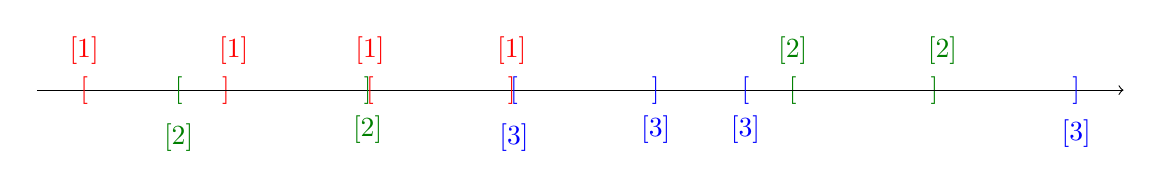
\begin{tikzpicture} [yscale=0.8,xscale=0.6] \node (O) at (0,0) {};

\draw[->] (0,0) -- (23,0);
 \draw (1,0) node[red] {$[$} node[above=0.2cm,red]
{$\ES[1]$}-- +(0:3cm)node[red] {$]$} node[right=0.1cm,above=0.2cm,red]{$\LS[1]$};

\draw(7.05,0) node[red] {$[$} node[above=0.2cm,red] {$\EE[1]$}-- +(0:3cm) node[red]
{$]$} node[above=0.2cm,red] {$\LE[1]$};
 \draw (3,0) node[Green] {$[$} node[below=0.3cm,Green]
{$\ES[2]$}-- +(0:4cm) node[Green] {$]$} node[below=0.2cm,Green] {$\LS[2]$};
 \draw
(16,0) node[Green] {$[$} node[above=0.2cm,Green] {$\EE[2]$}-- +(0:3cm) node[Green] {$]$}
node[right=0.1cm,above=0.2cm,Green] {$\LE[2]$};
 \draw(10.1,0) node[blue] {$[$}
node[below=0.3cm,blue] {$\ES[3]$}-- +(0:3cm) node[blue] {$]$} node[below=0.2cm,blue]
{$\LS[3]$};
 \draw (15,0) node[blue] {$[$} node[below=0.2cm,blue] {$\EE[3]$}--
+(0:7cm) node[blue] {$]$} node[below=0.25cm,blue] {$\LE[3]$};

\end{tikzpicture}
\end{center}

Après avoir trié les intervalles, nous obtenons:
$[\ES[1],\LS[1]] \le [\ES[2],\LS[2]] \le
[\EE[1],\LE[1]] \le [\ES[3],\LS[3]] \le 
[\EE[3],\LE[3]] \le [\EE[2],\LE[2]] $.

Alors, nous avons l'ensemble de contraintes suivantes:

\begin{itemize}
\item $t_2-t_1 \le \LS[2]-\ES[1]$
\item $t_3-t_2 \le \LE[1]-\ES[2]$
\item $t_4-t_3 \le \LS[3]-\EE[1]$
\item $t_5-t_4 \le \LE[3]-\ES[3]$
\item $t_6-t_5 \le \LE[3]-\EE[3]$
\end{itemize}

\end{ex}

Notons aussi que l'ensemble d'inégalités
$\underline{{\cal D}_e} \le t_e \le \overline{{\cal D}_e}$ peut ne pas
être valide. En effet, ici $t_6$ peut correspondre à la fin de
l'activité $3$ et $t_5$ à la fin de l'activité $2$, alors que
${\cal D}_5=[\EE[3],\LE[3]] \le [\EE[2],\LE[2]]={\cal D}_6$. On aurait
alors $\underline{{\cal D}_6} \le t_5 \le \overline{{\cal D}_6}$.

Ces contraintes peuvent être ajoutées au modèle on/off ou utilisées
comme borne supérieure sur la valeur de $\bmin(t_{e+}-t_e)$
dans~\eqref{bmin_CECSP_OO}. L'inégalité se réécrit donc comme:
\[ b_{ie} \ge \bmin(t_{e+}-t_e) - \bmin\left(\max(\overline{{\cal
D}_e},\overline{{\cal D}_{e+1}}) - \min(\underline{{\cal
D}_e},\underline{{\cal D}_{e+1}})\right)(1-z_{ie})\qquad \forall (i,e)
\in {\cal A}\times{\cal E}
\]

Ces inégalités peuvent être généralisées à tout sous-ensemble de $k$
intervalles ordonnés $\{{\cal D}_{e_1},\dots,{\cal D}_{e_k}\}$ avec
$t_{e_k}-t_{e_1} \le \max(\overline{{\cal D}_{e_1}},\overline{{\cal
D}_{e_k}}) - \min(\underline{{\cal D}_{e_k}},\underline{{\cal
D}_{e_1}}) $.

\paragraph{Date maximale d'un événement}


Une idée similaire à celle décrite dans le paragraphe précédent peut
être utilisée pour ordonner les événements et calculer des bornes
supérieures sur leur date. 

Pour faire cela, nous commençons par trier les bornes supérieures des
fenêtres de temps de chaque activité, i.e. $\LS$ et $\ES,\ \forall i
\in \A$, par ordre croissant. Alors, puisqu'un événement doit avoir
lieu dans chaque fenêtre de temps, i.e. avant chaque borne supérieure de
chaque fenêtre, nous pouvons déduire une borne supérieure sur la date
de chaque événement.

En effet, soit ${\cal UP}$ l'ensemble formé de toutes les bornes
supérieures de toutes les fenêtres de temps. Alors, nous avons la
propriété suivante: 
\begin{equation} \label {Bte_CECSP_OO} t_e \le {\cal UP}_e \qquad
\forall e \in {\cal E}
\end{equation}

\begin{ex} 
Considérons les intervalles définis dans
l'exemple~\ref{ex:evt_sep}. Alors, nous pouvons déduire l'ensemble de
contraintes suivantes:

\begin{itemize}
\item $t_1 \le \LS[1]$
\item $t_2 \le \LS[2]$
\item $t_3 \le \LE[1]$
\item $t_4 \le \LS[3]$
\item $t_5 \le \LE[2]$
\item $t_6 \le \LE[3]$
\end{itemize}
\end{ex}

Comme précédemment, nous pouvons utiliser ces inégalités comme
contraintes additionnelles des modèles à événements ou les utiliser
à la place de  $T$ dans les contraintes \eqref{twx_CECSP_OO}
et\eqref{twy2_CECSP_OO}. Les contraintes s'écrivent alors: 
\begin{align*}
& \ES z_{ie}\le t_e \le \LS(z_{ie}-z_{i,e-1})+(1-(z_{ie}-z_{i,e-1})){\cal UP}_e 
 & & \forall e \in \E\setminus \{1\},\ \forall i \in {\cal
   A}\\
&t_e \le \LE(z_{i,e-1}-z_{ie})+(1-(z_{i,e-1}-z_{ie})){\cal UP}_e  & & \forall e
 \in \E\setminus \{1\},\ \forall i \in {\cal
   A}
\end{align*}

Pour le \RCPSP, $t_n$ correspond à borne supérieure sur la durée
totale du projet, i.e. sur $T$.

\paragraph{Inégalités valides dérivées du problème de sac-à-dos}

Le rendement minimal de chaque activité pouvant être positif, nous
pouvons considérer les contraintes de type sac-à-dos suivantes pour
tout $e \in \Em$ et les transformer facilement en inégalités valides: 
\begin{equation}
\sum_{i\in \A^+} \bmin z_{ie} \leq B  \qquad  \forall e \in \E
\end{equation}
où $\A^+$ est le sous-ensemble d'activités avec $\bmin > 0$. 


\paragraph{Inégalités de cliques}

Les inégalités de clique permettent de modéliser le fait que plusieurs
variables binaires $z_{ie}$ ne peuvent prendre la valeur $1$
simultanément. Ces inégalités, déjà établies dans le cas du
\RCPSP~\cite{CAVT_clique}, correspondent aux sous-ensembles
disjonctifs d'activités. Elles sont facilement adaptables au cas du
\CECSP~et sont définies de la manière suivante. Soit $C$ un ensemble
minimal d'activités ne pouvant s'exécuter en parallèle, i.e. telles que
$\sum_{i \in C} \bmin > B$, alors l'ensemble d'inégalités suivantes
est valide pour le \CECSP: 
\begin{equation} 
\sum_{i\in C} z_{ie}  \le |C| -1 \qquad \forall C,\ \forall e \in \E
\end{equation}


Différentes techniques permettant l'intégration des inégalités
ci-dessus seront présentées et comparées dans le
chapitre~\ref{sec:expe}.

\chapter*{Conclusion}

Dans ce chapitre, nous avons présenté des modèles de programmation
linéaire en nombres entiers pour le problème du \RCPSP~ et pour le
\CECSP. Pour chacun de ces problèmes, trois modèles sont présentés,
un modèle utilisant une discrétisation de l'horizon de temps et deux
modèles basés sur une représentation des événements pertinents du
problème. 

Enfin, des améliorations de ces modèles sont proposées dans la
dernière partie du chapitre. Ces améliorations sont basées sur le
raisonnement énergétique, la mise en place d'inégalités valides et des
études polyédrales. De plus, les avantages et inconvénients de chacun
des modèles sont décrits ce qui permet de justifier l'intérêt de ces
améliorations. 

Des résultats numériques évaluant les performances de ces formulations
ainsi que l'intérêt de chaque amélioration sur diverses instances du
\CECSP~et du \RCPSP~feront l'objet d'un paragraphe dans le chapitre
portant sur les expérimentations (cf. Chapitre~\ref{sec:expe}). 